\documentclass{article}
\usepackage[UTF8]{ctex}
\usepackage[a4paper, total={6in, 8in}]{geometry}
\usepackage{graphicx}
\usepackage{float}
\graphicspath{{images/}}
\usepackage{booktabs}
\usepackage{enumitem}
\usepackage{amsmath}
\usepackage{amsfonts}
\usepackage{mathrsfs}
\usepackage{amssymb}
\usepackage{amsthm}
\usepackage{bm}
\usepackage{quantikz}
\usetikzlibrary{arrows.meta, positioning}
\usepackage{listings}
\usepackage{csquotes}
\usepackage{tabularx}
\usepackage{longtable}
\usepackage{ltablex}
\keepXColumns
\usepackage{caption}
\usepackage[colorlinks=true, linkcolor=blue, urlcolor=cyan]{hyperref}
\usepackage{xcolor}
\usepackage[most]{tcolorbox}

% ★★ 关键部分：启用 biblatex + biber ★★
\usepackage[backend=biber,style=numeric]{biblatex}
\addbibresource{references.bib}

\newtheorem{theorem}{Theorem}[section]
\newtheorem{lemma}[theorem]{Lemma}
\newtheorem{axiom}{Axiom}
\newtheorem{definition}{Definition}
\newtheorem{example}{Example}[section]

\tcbset{
   inlinehighlight/.style={
    on line,
    boxrule=0.5pt,
    colframe=orange!80!black,
    colback=orange!20,
    arc=2pt,
    boxsep=1pt
  }，
  highlightstyle/.style={
  enhanced,
  colback=yellow!10,
  colframe=orange!80!black,
  boxrule=0.5pt,
  arc=3pt,
  auto outer arc,
  fonttitle=\bfseries,
  boxed title style={
    colback=orange!30,
    colframe=orange!80!black
  }  
},
inlinebox/.style={enhanced, boxrule=0.5pt, colframe=orange!80!black, colback=orange!20, sharp corners, left=1pt, right=1pt, top=1pt, bottom=1pt, boxsep=0pt, arc=2pt, before skip=0pt, after skip=0pt, frame hidden=false, on line}
}

\title{My Note of Studying the Quantum Computation}
\author{Ye Ning}
\date{July， 05， 2025}

\begin{document}

\maketitle

\tableofcontents

\section{Introduction}
This is a draft of an informal note, a summary of what I read recently about the quantum computing, especially on the topic of so-called Quantum Variational Eigensolver (QVE). In this note, I included not only some discussions over the material I read, but also my own thoughts and comments even if they are immature. I plan to mark the unanswered questions in this note if there is any. Python code is presented here in form of listing.

For now, this note is not organized logically, some material and idea are included in an ad hoc way. But I believe, given more time, with the accumulation of reading and discussion, this note will become informative, formal and satisfying. Hopefully, I wish this note can be eventually developed into a self-contained, well-organized reference book for the future researchers and/or lecturers.
\section{The Variational Quantum Eigensolver (VQE)}
\subsection{Overview of VQE}
VQE~\cite{IBMQuantumVQE, Abhijith2018QuantumBeginner, Peruzzo2014VQE} is an algorithm that uses classical and quantum computing in conjunction to accomplish a task.  Usually, the VQE is composed of four parts: an operator, an ``ansatz", an estimator and a classical optimizer. The operator is often a Hamiltonian $\mathcal{H}$, that describes the property of the system we are studying. We need to use the variational method to figure out the eigenvector of the operator to minimize the eigenvalue. The ansatz is actually a quantum circuit that prepares a quantum state approximating the eigenvector we are seeking. The gates in the ansatz are parametrized, and we can vary those parameters iteratively to achieve the minimum expection value. The estimator is a means of estimating the expectation value of the opertor $\mathcal{H}$ over the current quantum state. In the following question we are dealing with (the quantum chemical computation see section~\ref{section:AdaptiveGridMethod}),  the ultimalte result that I care about is the expectiona value, which is related to the eigenvaluees (energy level) of the system, and this expectation value is also called the cost function.   

Before the invention of VQE, the quantum approach to eigenvalue problem is quantum phase estimation (QPE). In this algorithm, the eigenvector $\ket{\psi}$ of a Hermitian operator $\mathcal{H}$ is regarded as input and the problem is to calculate the corresponding eigenvalue $\lambda$, which is determined by successive application of $e^{-i\mathcal{H}t}$ onto $\ket{\psi}$. However, this method needs millions or billions of quantum gates for practical application while only tens to hundreds of gates are available right now. 

To overcome this difficulty, VQE is introduced to solve the eigenvalue problem by figuring out the $\ket{\psi}$ that can minimizes the so-called Rayleigh-Ritz quotient:
\begin{equation}
    \frac{\bra{\psi}\mathcal{H}\ket{\psi}}{\langle\psi\ket{\psi}},
\end{equation}
via a variational method. To realize the quantum computation, the Hamiltonian can be written into the second quantization form:
\begin{equation}
    \mathcal{H}=\sum_{p,q}h_{pq}a^\dagger_pa_q+\frac{1}{2}\sum_{p,q,r,s}h_{pqrs}a^\dagger_pa^\dagger_q a_r a_s,
    \label{eqn:secondQuantizedHam}
\end{equation}
where $a^\dagger_p$ and $a_p$ are fermionic creation and annihilation operators, respectively. The real numbers $h$'s are one- or two-electron integrals that can be easily computed on a classical computer. Then this formulation should be further mapped onto a quantum computer to calculate
\begin{equation}
    \label{secondQuantizedH}
    \mathcal{H}=\sum_{i\alpha}h^i_\alpha\sigma^i_\alpha + \sum_{ij\alpha\beta}h^{ij}_{\alpha\beta}\sigma^i_\alpha\sigma^j_\beta+\dots.
\end{equation}
 Here Latin indices identify the subsystem on which the operator acts, and Greek indices identify different type of Pauli operators. For now, there are three different mapping schemes, and the mapping process will be discussed further below. Regardless the choice of mapping method, the equation above sometimes is written as
 \begin{equation}
    \mathcal{H}=\sum_j\alpha_j P_j=\sum_j\alpha_j\prod_\alpha\sigma_\alpha^j,
 \end{equation}
 where $\alpha_j$ are real scalar coefficients depend on the $h$s, and $P_j$ are called Pauli words (strings), representing a product of Pauli matrices.
 Based on the equation (\ref{secondQuantizedH}), the expectation value of $\mathcal{H}$ is expressed as:
 \begin{equation}
    \langle\mathcal{H}\rangle=\sum_{i\alpha}\langle\sigma_\alpha^i\rangle+\sum_{ij\alpha\beta}\langle\sigma_\alpha^i\sigma_\beta^j\rangle+\dots.
 \end{equation}
 The following snippet of Python code is from~\cite{IBMQuantumVQE}, demonstrating how the operator is presented as code:
 \begin{lstlisting}[language=Python, caption=Constructing an Operator for VQE, frame=single, label={lst:Constructing Operator}]
from qiskit.quantum_info import SparsePauliOp
 
hamiltonian = SparsePauliOp(
    [
        "IIII",
        "IIIZ",
        "IZII",
        "IIZI",
        "ZIII",
        "IZIZ",
        "IIZZ",
        "ZIIZ",
        "IZZI",
        "ZZII",
        "ZIZI",
        "YYYY",
        "XXYY",
        "YYXX",
        "XXXX",
    ],
    coeffs=[
        -0.09820182 + 0.0j,
        -0.1740751 + 0.0j,
        -0.1740751 + 0.0j,
        0.2242933 + 0.0j,
        0.2242933 + 0.0j,
        0.16891402 + 0.0j,
        0.1210099 + 0.0j,
        0.16631441 + 0.0j,
        0.16631441 + 0.0j,
        0.1210099 + 0.0j,
        0.17504456 + 0.0j,
        0.04530451 + 0.0j,
        0.04530451 + 0.0j,
        0.04530451 + 0.0j,
        0.04530451 + 0.0j,
    ],
)
\end{lstlisting}
The listing above describes a $16\times16$ Hamiltonian matrix. The reason is that the length of each Pauli string, such as \tcbox[inlinebox]{IIII}, or \tcbox[inlinebox]{YYYY}, is four. For a $n$-bit Hilbert space, its dimension is $2^n$. Therefore, for $n=4$, its dimensionality is $2^4=16$. Besides, in the \tcbox[inlinebox]{SparsePauliOp} class, those Pauli strings and coefficients are strictly one-to-one related. Take the second Pauli string \tcbox[inlinebox]{IIIZ} as an example, its corresponding coefficient is \tcbox[inlinebox]{-0.1740751}. Considering \tcbox[inlinebox]{IIIZ} is a 4 qubits Pauli tensor product:
\[
"IIIZ"=I\otimes I\otimes I\otimes Z,
\]
this Pauli string/coefficient pair denotes $-0.1740751\cdot(I\otimes I\otimes I\otimes Z)$.

In~\cite{IBMQuantumVQE}, we can also read of the comments of the listing above like:
\begin{quote}
    Note that in the Hamiltonian above, there are terms like ZZII and YYYY that do not commute with each other. That is, to evaluate ZZII, we would need to measure the Pauli Z operator on qubit 3 (among other measurements). But to evaluate YYYY, we need to measure the Pauli Y operator on that same qubit, qubit 3. There is an uncertainty relation between Y and Z operators on the same qubit; we cannot measure both of those operators at the same time.
\end{quote}
In this quotation, we can see there is a problem concerning the measuements of the uncommutative operators. So, how to solve the problem? The answer to this question is: measurement in batches. That means we do not perform the measurements simmultaneous, instead, in every batch of measurement the quantum state will be appropriately rotated to $Z$ basis if necessary, since quantum computer can only measure $Z$ basis. For example, if we want to measure $Y$, we must rotate $Y$ into $Z$:
\[
Y = R_x\!\left(-\frac{\pi}{2}\right) Z R_x\!\left(\frac{\pi}{2}\right).
\]
After measured upon $Z$, the result will be interperated as measurement upon $Y$. This method does not vilote the priciple of uncertainty, since we do not perform the measurement simultaneously. Instead, for each batch of the measurement, we prepare the same input state. To realize the batch measurement efficiently, we need to catogarize the Pauli strings wisely to decrease the times of measuring. Since it is more like an engineering problem, details of this issue will not be mentioned here.

Now, let's learn something about ansatz. In~\cite{IBMQuantumVQE}, we are given an ansatz like the figure below.
\begin{figure}[ht]
\centering
    \begin{quantikz}
        \lstick{$\ket{0}$} & \gate{R_y(\theta_0)} & \ctrl{1} & \qw & \ctrl{1} & \gate{R_y(\theta_3)} & \qw \\
        \lstick{$\ket{0}$} & \gate{R_x(\theta_1)} & \targ{} & \gate{R_z(\theta_2)} & \targ{} & \gate{R_x(\theta_4)} & \qw
    \end{quantikz}
\caption{Five-Step Ansatz}
\label{fig:FiveStepAnsatz}
\end{figure}
If we want to know the functionality of this circuit, we need to read it column by column like we are reading a piano music staff. Suppose those two lines corresponging to qubits, qubit 0 is the upper one and the qubit 1 is the lower one. Both of them are initialized as $|0\rangle$ From the left to the right, the first column is 
\[
U_1=R_y^{(0)}(\theta_0)\otimes R_x^{(1)}(\theta_1);
\]
the second column is only a CNOT, which can be expressed as:
\[
U_2=\text{CNOT}_{0\rightarrow1};
\] 
The unitary operator for the third column is
\[
U_3=I^(0)\otimes R_z^{(1)}(\theta_2);
\]
and it is obvious that $U_4=U_2=\text{CNOT}_{0\rightarrow1}$. For column 5, its unitary operator is
\[U_5=R_y^{(0)}(\theta_3)\otimes R_x^{(1)}(\theta_4).\]
Therefore, the total unitary operator of the circuit is
\begin{equation}
    U(\theta)=U_5U_4U_3U_2U_1.
\end{equation}
The middle three terms, 
\begin{equation}
    U_{\text{mid}}=U_4U_3U_2=\text{CNOT}\left(I\otimes R_z(\theta_2)\right)\text{CNOT},
    \label{eqn:MiddleThree}
\end{equation}
 can be simplified via the standard identity $\text{CNOT}\left(I\otimes Z\right)\text{CNOT}$, which can be applied to the case of rotation as $\text{CNOT}\left(I\otimes R_Z(\theta_2)\right)\text{CNOT}=e^{-i\frac{\theta_2}{2}Z\otimes Z}$. Therefore, the whole circuit can be expressed as:
 \begin{equation}
    U(\theta)=\left(R_y^{(0)}(\theta_3)\otimes R_x^{(1)}(\theta_4)\right)e^{-i\frac{\theta_2}{2}Z\otimes Z}\left(R_y^{(0)}(\theta_0)\otimes R_x^{(1)}(\theta_1)\right).
 \end{equation}
 Now, the question we need to answer is that since we can simplify this expression, why cannot we construct a controlled rotation circuit directly rather than such a sandwich structure? The answer is: such a sandwich structure is hardware friendly since most superconductive quantum chips such as IBM Quantum cannot excecute arbitary angle controlled rotation directly. Plus, in a variational circuit, such a structure can generate entanglement between two qubits effectively, while $\theta_2$ can be used to decide the ``strength'' of the entanglement.
 
\subsection{ADAPT-VQE}
ADAPT-VQE  is a smart greedy algorithm. However, it constructs the ansatz by including the exciting operators (single-excitation, double-excitation) in a term-by-term manner (organically growth). For each step of including a new term, the purpose is to maximize the energy drop (energy gradient), regardless whether if it is a violation of the symmetry of the system. As a result, it can give rise to a low-energy but non-physical state, such as violating the conservation of particle number or spin symmetry.
\subsection{Valence Bonding}
The first formula in \cite{UnbChemistry} is like
\begin{equation}
     |H_2\rangle= \cos(\frac{\theta}{2})|\sigma\bar{\sigma}\rangle+\sin(\frac{\theta}{2})|\sigma^*\bar{\sigma}^*\rangle, 
     \label{valenceBonding}
\end{equation}
where $\sigma $ means bonding and $\sigma^*$ means anti-bondig orbital. The bar used here means that the electron in this orbital is spin-down. Therefore, $|\sigma\bar{\sigma}\rangle$ denotes a pair of bonding orbital electrons, one spin-up, the other spin-down. In other words, those symbols are used to clearly label in which orbit the electron is in and its spin direction. 
In this formula, $\cos(\frac{\theta}{2})$ and $\sin(\frac{\theta}{2})$ are two important parameterized coefficients, as they reflect \textbf{the proportionality of quantum superposition} of the bonding orbital states and antibonding obital states. In other words, those two parameters control whether the electrons tend to the ``stable combination'' or to the ``exited combination'' of the chemical bonds. $|\sigma\bar{\sigma}\rangle$ denote that the two electrons are in the $\sigma$ orbital (bond-forming orbital), forming the stable covalence bond. Meanwhile, $|\sigma^*\bar{\sigma}^*\rangle$ is an unstable state. The superposition of those two states gives rise to a more flexible and adjustable wavefunction. The reason that we use the single $\theta$ rather than two independent parameters is that by doing so we can guarantee the automatic normalization of the wave functions, which is $\cos^2\frac{\theta}{2}+\sin^2\frac{\theta}{2}=1$. This is a quantum-circuit-friendly expression which means, it can be easily mapped into a rotation gate.

For a single qubit, the application of the rotation gate on a $\ket{0}$ is as follows:
\begin{lstlisting}[language=Python, caption=Sample Python Code, frame=single]
from qiskit import QuantumCircuit
from qiskit.circuit.library import RYGate

theta = 1.2  # Define angle
qc = QuantumCircuit(1)
qc.ry(theta, 0)  # Or use: qc.append(RYGate(theta), [0])
qc.draw()
\end{lstlisting}

% \begin{figure}[h]
%     \centering
%     \begin{quantikz}
%         \lstick{$\ket{0}$} & \gate{RY(\theta)} & \qw
%     \end{quantikz}
%     \caption{Caption}
%     \label{fig:enter-label}
% \end{figure}
    
\begin{equation}
    \begin{quantikz}
        \lstick{$\ket{0}$} & \gate{RY(\theta)} & \qw
    \end{quantikz},    
\end{equation}
and matrix form of the single qubit rotation gate is:
\begin{equation}
    R_Y(\theta)=\begin{bmatrix}
    \cos(\frac{\theta}{2}) & -\sin(\frac{\theta}{2}) \\ \sin(\frac{\theta}{2}) & \cos(\frac{\theta}{2})
    \end{bmatrix}
\end{equation}
Therefore, assume the initial state of a qubit is $\ket{0}=\begin{bmatrix}1\\0\end{bmatrix}$, then after the rotation via the gate, it turns out to be 
\begin{equation}
    \ket{\psi}=R_Y(\theta)\ket{0}=\begin{bmatrix}
        \cos(\frac{\theta}{2}) \\ \sin(\frac{\theta}{2})
    \end{bmatrix} = \cos(\frac{\theta}{2})\ket{0}+\sin(\frac{\theta}{2})\ket{1},
\end{equation}
which is exactly the wavefunction of a hydrogen molecule. 

The following formula is Eq. (4) in \cite{UnbChemistry}. 
\begin{equation}
    \begin{quantikz}
\lstick{\ket{0}} & \gate{RY(\theta_0)} & \ctrl{1} & \qw \\
\lstick{\ket{0}} & \gate{RY(\theta_1)} & \targ{}  & \qw
\end{quantikz}
\end{equation}
Its corresponding Qiskit should be:
\begin{lstlisting}[language=Python, caption=Sample Python Code, frame=single]
from qiskit import QuantumCircuit
import numpy as np

theta = 1.2  # 可任意调整角度
qc = QuantumCircuit(2)
qc.ry(theta, 0)  # θ₀ = θ
qc.ry(np.pi, 1)  # θ₁ = π
qc.cx(0, 1)
qc.draw('mpl')
\end{lstlisting}
Functionality of each part:
\begin{itemize}
    \item \tcbox[inlinebox]{$R_Y(\theta)$}: Exerting Y-axis rotation on the first qubit, constructing the linear superposition of $\ket{\sigma}$ and $\ket{\sigma^*}$.
    \item \tcbox[inlinebox]{$R_Y(\pi)$}: rotating the second qubit to its ground state $\ket{1}$, corresponding to the spin-down electron.
    \item \tcbox[inlinebox]{$CNOT(0\rightarrow1)$}: introducing the entanglement, forming the\textbf{ resonant mixed state} rather than the simple multiplication state of the electron, which is exactly the superposition relation reflected in Eq. \ref{valenceBonding}.
\end{itemize}

\subsection{Mapping Methods}
\label{sec:MappingMethods}
In the following three subsections, we briefly describe an essential process in quantum computation -- mapping. Actually, the process is one of the fundamental difference between the quantum computation and the classical computation. Of course, this process requires extra over-head or even some sophisticated algorithms.  

First, we need to explain why we need this procedure. Unlike the classical system, qubit cannot be read without wavefunction collapse. For this reason, ``parity'' should be coded rather than being stored. It should manifest itself naturally in the state evolvement process. For the same reason, keeping the anti-commutativity of the fermionic operators must be a ``measurement-free'' structural operation, requiring the automatic change of the sign.  This requirement can only be achieved by the dynamic construction process of the qubit gates, not the afterward correction by classical bits. In addition, the advantage of quantum computation is essentially based on quantum entanglement and quantum superposition, while in many scenarios, parity is tightly related to the entangled structure. Therefore, parity, as an important quantum feature, is not a certain value that can be stored by a classical bit. For example, in the following superposition state,
\begin{equation}
    \ket{\psi}=\frac{1}{\sqrt{2}}(\ket{0100}+\ket{1011}),
\end{equation}
one cannot tell electron is in which orbital exactly, since the coexistence of the two states. Parity is decided by the ``number of the electrons in certain interval'', and this number can only be obtained from  measurement after the collapse of the wavefunction.

Meanwhile, in the framework of second quantization, a fermionic orbit can be either vacant or occupied, similar to the classical bit (0 or 1). As we know, the qubit can only be either $\ket{1}$ or $\ket{0}$ or their superposition, therefore, it is nature to use a qubit to represent a fermionic orbit. This in turn makes it feasible to map a fermionic Hamiltonian into a qubit Hamiltonian, hence the algorithms like VQE or QPE.

To this end, we define three types of set, and one of the important tasks of mapping schemes is to update those sets correctly:
\begin{table}[ht]
\centering
\caption{Three Key Sets in Bravyi--Kitaev Mapping}
\label{tab:bksets}
\begin{tabular}{|l|p{0.7\linewidth}|}
\hline
\textbf{Set} & \textbf{Description} \\
\hline
Update set & Qubits that must be flipped when a mode changes. \\
Parity set & Tracks parity of modes before the current one. \\
Occupation set & Tracks whether a mode is occupied. \\
\hline
\end{tabular}
\end{table}


\subsubsection{Jordan-Wigner Mapping (JWM)}
Jordan-Wigner mapping is used to convert Fermion operator into spin operator such as Pauli matrix. At first, it was established to solve 1-D spin chain model, but now it is widely used in quantum chemistry and quantum physics simulation. Its key idea is to map each orbital in the Fermion system to a qubit, and use Pauli matrix to represent Fermion operator, without changing the anti-commute property.
Here is a simplified version of mapping formula:
\begin{equation}
    a^\dagger_j=\left(\prod_{k=0}^{j-1}Z_k\right)\cdot \frac{X_j-iY_j}{2},
    \label{simplifiedJWM}
\end{equation}
where $X_j, Y_j, Z_j$ are the $j^{th}$ qubit on the Pauli matrix. $\prod_{k=0}^{j-1}Z_k$ is also called the \textbf{Z chain}, its functionality is to guarantee that when we exchange the Fermions, a  negative sign can be correctly introduced so that the overall anti-commutativity is maintained. Please note, in the equation above, when $k=0$, we follow the rule: 
\begin{equation}
    \prod_{\text{empty product}}=1.
\end{equation} 
The anti-commutation relations are:
\begin{equation}
\begin{aligned}
    \{a_i,a_j\} &= a_ia_j+a_ja_i \\
    \{a^\dagger_i, a^\dagger_j\} &= 0 \\
    \{a_i, a^\dagger_j\} &= \delta_{ij}
\end{aligned} 
\label{eqn:anti-comm}
\end{equation}
When we are going to map the fermionic operator to the Pauli matrix, we need to keep the anti-commutativity structure. In Jordan-Wigner mapping, the operator on the $j^{th}$ orbital can be expressed as:
\begin{itemize}
    \item Creation Operator:
    \begin{equation}
        a^\dagger_j=\left(\prod_{k=0}^{j-1}Z_k\right)\cdot\frac{X_j-iY_j}{2}        
    \end{equation}
    \item Annihilation Operator:
    \begin{equation}
        a_j=\left(\prod_{k=0}^{j-1}Z_k\right)\cdot\frac{X_j+iY_j}{2} ,     
    \end{equation}
\end{itemize}
It is obvious that when the system is complex enough, the Z chain will be very long which causes a deep circuit. Luckily, this in NOT the only way to maintain the overall anti-commutativity. There are two well-known methods can address the anti-commutativity more efficiently. They are \textbf{Parity Mapping} and \textbf{Bravyi-Kitaev Mapping}.

\subsubsection{Parity Mapping}
Rather than ``memorizing how may Fermion are there on the left side of the orbital'', the Parity Mapping method records the ``Parity'' directly. Its creation operator is like:
\begin{equation}
    a^\dagger_j=\left(\prod_{k\in P(j)}Z_k\right)\cdot\frac{X_j-iY_j}{2},
\end{equation}
where $P(j)$ is the orbital collection related to the $j^{th}$ orbital, used to guarantee the anti-commutativity. The advantage of this idea is this mapping method does not need the Z chain get longer with the increment of the orbital number. On the contrary, it may become shorter. It can keep the symmetrical property of the system better under some circumstances, such as the projection of spins. However, this mapping strategy is not so straightforward as the JWM, so that the Parity Mapping process is more complicated and harder to debug than JWM.  

\subsubsection{Bravyi-Kitaev Mapping (BKM)}
%\subsubsection{\texorpdfstring{Bravyi-Kitaev Mapping (BKM)~\cite{transfer2015BKmapping}}{Bravyi-Kitaev Mapping (BKM)}}
This is a more sophisticated mapping method, which distribute information to many qubits. It can track down the \textbf{local occupation} and the \textbf{accumulation of parity} at the same time. It uses a balanced way to encode the anti-commutativity into the circuit to achieve the following two competing goals:
\begin{itemize}
    \item \textbf{Locality}: minimizing how many qubits a single fermionic operator affects.
    \item \textbf{Efficiency}: reducing the number of quantum gates needed to simulate fermionic interactions.
\end{itemize}
To achieve those goals, \textbf{binary tree structure} is used to encode both \textbf{occupation} and \textbf{parity} information, allowing it to update fewer qubits when simulating fermionic creation/annihilation operators.

Specifically, BKM updates three key sets listed in Table~\ref{tab:bksets} via a transformation matrix, and this transformation matrix is set up in a recursive manner. This leads to a more compact and efficient representation of the system's Hamiltonian.

In this method, we need to generate a so-called Bravyi-Kitaev basis ($\vec{b}_n$) from the occupation state vector ($\vec{f}_n$) via a square transformation matrix $\beta_n$ such that $\beta_n\vec{f}_n=\vec{b}_n$. The matrix $\beta_n$ is constructed in a recursive manner:
\begin{equation}
    \beta_{2^x}=\left[\begin{array}{c|c}
        \beta_{2^{x-1}} & 0 \\
        \hline
        \begin{matrix}
            0\\ \leftarrow 1 \rightarrow
        \end{matrix} & \beta_{2^{x-1}}
    \end{array}
        \right] \qquad \text{where} \: \beta_1=\left(1\right)
\end{equation}
Let's repeate the example in~\cite{transfer2015BKmapping}, for eight qubits, $\beta_n\vec{f}_n=\vec{b}_n$ is specified into (\textcolor{red}{all sums in mod(2)}): 
\begin{equation}
    \label{8bits}
    \begin{bmatrix}
        1&0&0&0&0&0&0&0\\
        1&1&0&0&0&0&0&0\\
        0&0&1&0&0&0&0&0\\
        1&1&1&1&0&0&0&0\\
        0&0&0&0&1&0&0&0\\
        0&0&0&0&1&1&0&0\\
        0&0&0&0&0&0&1&0\\
        1&1&1&1&1&1&1&1
    \end{bmatrix}
    \begin{bmatrix}
        f_0\\f_1\\f_2\\f_3\\f_4\\f_5\\f_6\\f_7
    \end{bmatrix}
    =
    \begin{bmatrix}
        f_0\\f_1+f_0\\f_2\\f_3+f_2+f_1+f_0\\
        f_4\\f_5+f_4\\f_6\\f_7+f_6+f_5+f_4+f_3+f_2+f_1+f_0
    \end{bmatrix}.
\end{equation}
From the right side of Eq.~\ref{8bits}, we can figure out the rules for constructing Update Set. If the occupation state of the first orbit is changed, then those need to be updated components of $\vec{b}_n$ are $b_0, b_1, b_3$ and $b_7$, not all of them. Similarly, when $f_1$ is changed, the Update Set contains only $b_1$, $b_3$ and $b_7$. We don't need to consider components with even label in $\vec{b}_n$, since those items contain only the occupation state of that orbital itself, and in the Update Set, the orbital itself is NOT included. If we want to construct Update Set $U(j)$, then $b_0$ to $b_j$ need not be checked, since those components do not contain the information of orbital $j$. The reason is the transformation matrix is a lower triangular matrix. For example, if $f_3$ is changed, $b_0$, $b_1$ and $b_2$ will not be affected.

Given the $\vec{f}_n$, to figure out the Parity Set is not a difficult job, as long as we make use of matrix
\begin{equation}
    [\pi_n]_{ij}=\begin{cases}
        1, & \qquad \text{if} \; i<j \\
        0, & \qquad \text{otherwise}
    \end{cases}.
\end{equation}
Then $\pi_n \vec{f}_n$ will give us the Parity Set.

The analysis above tells us if we have already known the $\vec{b}_n$, then we can obtain occupation bais by $\beta_n^{-1}\vec{b}_n=\vec{f}_n$, and by multiplying $\pi_n\beta_n^{-1}$ on the Bravyi-Kitaev basis we can find out the parity.

Once again, using eight qubits as an example, we can see 
\begin{equation}
    \beta^{-1}_8=
    \begin{bmatrix}
        1&0&0&0&0&0&0&0\\
        1&1&0&0&0&0&0&0\\
        0&0&1&0&0&0&0&0\\
        0&1&1&1&0&0&0&0\\
        0&0&0&0&1&0&0&0\\
        0&0&0&0&1&1&0&0\\
        0&0&0&0&0&0&1&0\\
        0&0&0&1&0&1&1&1
    \end{bmatrix}.
\end{equation}
And again, this reverse matrix can be constructed from a recursive relation:
\begin{equation}
    \beta_{2^x}=
    \left[\begin{array}{c|c}
        \beta_{2^{x-1}}^{-1} & 0 \\
        \hline
        0_1 & \beta_{2^{x-1}}^{-1}
    \end{array}\right] 
    \qquad \text{where} \: \beta_1^{-1}=\left[1\right]
\end{equation}
\vspace{0.5em}
\hrule
\vspace{0.5em}
\textit{\textbf{Reflection:} Although the discussion above shows the effectiveness of the one-orbit-to-one-qubit mapping method, it may not be the only solution to current situation, and it is potentially problematic. First, it suffers from ``over-abstraction'', which means after the complicated electron wave functions are compressed into binary occupation states, the information about symmetry, entanglement and group structure may be lost. What make things worse is the risk of generating non-physical states, such as the state that violate the conservation of spin, etc. Many body wave function is more than a simple combination of the orbital occupation, it also contains coupling and correlation between the states, which cannot be covered perfectly only by qubits.}

\textit{To overcome those defects, people are thinking of other solutions. For example, Tensor Network Quantum Simulation (TNQS) \cite{TensorNetwork}  does not use ``orbit occupation'' as the fundemental block, instead, it uses an entangled structure to describe the whole wavefunction. Group-equivariant Ansatz (GEA) uses group structure to construct variational state. Quantum Natural Orbitals plus Subspace Encoding method makes use of classical calculation to obtain the principle orbitals and then encode the subspace state. Bosonic or Fermionic Simulation Framework skip over the step of orbital mapping, it uses qubit to denote the vector or the symmetrical spatial wavefunction.}



\subsection{Measuring the Qubit Circuit}
Suppose we have
\begin{equation}
    \langle H\rangle =\sum_i h_i\bra{\psi}P_i\ket{\psi},
\end{equation}
where $P_i$ is the Pauli words like $X_0Y_1Z_2$,  the $h_i$ is the corresponding real coefficient, and $\ket{\psi}$ is the current output ansatz quantum state. Then the question is how to measure $\bra{\psi}P_i\ket{\psi}$ in the qubit circuit?

Now, take Pauli words $P_i=Z_0Z_1$ as an example, we need to take the following steps to measure:
\begin{enumerate}
    \item \textbf{Preparing the state}: Use the variational circuit to generate $\ket{\psi}=U(\bar{\theta})\ket{0\dots0}$.
    \item \textbf{Choosing the measuring base}: For example, if we want to measure $Z_0Z_1$, we need to perform Z base measurement on the $0th$ and the $1st$ qubit, which is the default measurement. Once we get two results $m_0, m_1\in\{+1, -1\}$, we calculate product $m_0\cdot m_1$. Except the default measurement, to perform other types of measurements, we need to add base conversion gate before the measurement:
    \begin{table}[h!]
        \centering
        \caption{Base Conversion Gate}
        \label{tab:BaseConversion}
        \begin{tabular}{c|l}
        \toprule
          The target Pauli word   & The corresponding gate to be added \\
        \midrule
            X & Hadamard gate \\
            Y & $S^\dagger+$ Hadamard gate \\
            Z & Don't need to add any gate \\
        \bottomrule
        \end{tabular}
    \end{table}
    \item \textbf{Repeating measurement and calculating the average value}: We need to repeat the measurement of $P_i$ many times to get many samples (shots), say 1024 times, to obtain average value of product:
    \begin{equation}
        \langle P_i\rangle \approx \frac{1}{N}\sum_{j=1}^N m_0^{(j)}\cdot m_1^{(j)}\cdot\dots ,
    \end{equation}
    then we multiply this by $h_i$ to obtain the contribution to the energy from this term.
\end{enumerate}
The relevant Qiskit code can be found in Listing~\ref{lst:CircuitMeasure}.

\subsection{Transverse-Field Ising Model}
The \textbf{Transverse-Field Ising Model} referred to in \cite{UnbChemistry} is a typical quantum spin model, which is widely used in the study of quantum phase transition, entanglement, and the design of the variational algorithm in the quantum computation.

For the 2-site system, \cite{UnbChemistry} shows that the Hamilton as:
\begin{equation}
    \hat{H}_{2-site}=-JZ_0Z_1-h(X_0+X_1), 
\end{equation}
where:
\begin{itemize}
    \item $Z_i$, $X_i$ are the Pauli-Z and Pauli-X operator on the ith qubit.
    \item $J$ is the coupling strength between spins (along the $Z$ direction).
    \item $h$ is the strength of the transverse magnetic field (along the $X$ direction).
\end{itemize}
The first term, $-JZ_0Z_1$, tends to (anti)align the neighboring spin along the z-direction, describing the spin interaction. The second term, $-h(X_0+X_1)$, introduces the transverse magnetic field, makes the spin flip along the X-direction, describes the quantum fluctuation. Competition between those two terms gives rise to the quantum phase transition, which means the system changes from the ordered state (spin aligns) to the disordered state (spin flips).
\subsection{One-shot Calculation}
One-shot calculation means in VQE, a complete calculation is performed upon a certain set of parameters without referring to previous results of those parameters in the course of the ``continuous evolvement''.

More specifically, in \cite{UnbChemistry}, there are two optimization strategies:
\begin{enumerate}
    \item Default strategy \begin{itemize}
        \item Each calculation starts with a randomly initialized angle;
        \item Every parameter, such as length of bond, different model parameters, will be optimized independently.
        \item Pros: One can jump to any point in the parametric space without worrying about the history.
        \item Cons: It is easy to get stuck in the local minimum, especially in a complex system.
    \end{itemize}
    \item Adiabatic strategy \begin{itemize}
        \item Start from a relative easier parameter, such as the balance bonding length.
        \item Then change the parameters gradually, each new iteration starts with the optimized parameter from the previous circle.
        \item Pros: More stable, unlikely to get stuck in local minimum;
        \item Cons: Cannot jump to any point easily, one must ``cover the whole path''.
    \end{itemize}
\end{enumerate}
\section{Use of the Basis}

\subsection{\href{https://en.wikipedia.org/wiki/STO-nG_basis_sets}{STO-nG}}
STO-nG is a short of ``\textbf{S}late-\textbf{T}ype \textbf{O}rital with \textbf{n} \textbf{G}aussians'', and the STO-3G is the simplest of the set. Take the STO-3G as an example, its main idea is to use 3 Gaussians to fit an approximate Slater type of orbital. There is a two-fold motivation behind this. One is that the STO is very close to the real atomic orbital shape but needs complicated computation; the other is that the Gaussians are efficient in calculation. Therefore, this scheme balances the physical precision and the computational efficiency.

Mathematically, every atomic orbital (such as $1s$, $2s$ and $2p$) can be expressed as:
\begin{equation}
    \phi_{\text{STO-3G}}=\sum_{i=1}^3 c_i\cdot\phi_{\text{GTO}}(\alpha_i),
\end{equation}
where $c_i$ is the coefficient of each GTO, $\alpha_i$ is the exponential index of each GTO. All the GTO are the radial wavefunctions centered on the nuclear. Usually, those parameters are obtained via the least squares method.

Taking the hydrogen molecule as an example, we can construct a complete quantum Hamiltonian for it step by step. First, we need to use tools like  \textit{Qiskit Nature} or \textit{PySCF} to decide geometry such as internuclear distance, such as 0.74 \text{\AA}, which is close to ground state. Then the basis STO-3G is chosen. After that, we need to initiate the Hartree-Fock calculation to obtain the single- and double- electron integration. Under STO-3G, two $1s$ orbitals (one for each hydrogen atom) are used. After Hatree-Fock, we get Hamiltonian like:
\begin{equation}
    \hat{H}=\sum_{pq}h_{pq}a^\dagger_pa_q+\frac{1}{2}\sum_{pqrs}h_{pqrs}a^\dagger_pa^\dagger_qa_ra_s.
\end{equation}
Therefore, we obtain four (spin) orbitals: 2 spatial orbitals times $\alpha, \beta$ spin leads to 4 fermionic up/down operator indices. We can now map the Hamilton into Pauli words by using either JWM or BKM. Taking JWM as an example, the mapping leads to:
\begin{equation}
    H=c_0I+c_1Z_0+c_2Z_1+c_3Z_0Z_1+c_4Y_0X_1X_2Y_3+\dots,
\end{equation}
in which every term such as $Z_0Z_1$, $Y_0X_1X_2Y_3$ etc. are measurable Pauli words, and each corresponding to a coefficient $c_i$. Those coefficients are the result of the collection of molecular integration after the anti-commutative expansions. The related Qiskit code is demonstrated in Listing~\ref{lst:HamiltonGeneration}.

Now, let us take a closer look at the STO-3G for hydrogen molecule. As mentioned before, for each of the hydrogen atom, it approximate Slater orbital is:
\begin{equation}
    \phi_{\text{STO}}=Ne^{-\zeta r},
\end{equation}
and in STO-3G, this $1s$ orbital is approximately expressed as a linear comibination of 3 GTO:
\begin{equation}
    \phi^{\text{STO-3G}}_{1s}(r)=\sum_{i=1}^3 c_i\cdot\phi^{(i)}_{\text{GTO}}(r).
\end{equation}
More specifically, in spherical coordinate, a standard GTO is:
\begin{equation}
    \phi^{(i)}_{\text{GTO}}(r, \theta, \phi)=N_i\cdot Y_{l,m}(\theta,\phi)\cdot r^{2n}e^{-\alpha_i r^2},
\end{equation}
where $N_i$ is the normalization factor, $Y_{l,m}$ is the spherical harmonic function for the angular part, $r^{2n}$ is the polynomial radial part ($n=0$ is for the $1s$ orbital), $\alpha_i$ is the $i^{th}$ GTO Gaussian Index. As an example, for the $1s$ orbital of hydrogen, the angular part is $Y_{0,0}=\frac{1}{\sqrt{4\pi}}$, which is a constant, reflecting the fact that the $s$ orbital is isotropic. The radial part is $r^0=1$. Therefore, every GTO is simplified into
\begin{equation}
    \phi^{(i)}_{\text{GTO}}=N_i\cdot e^{-\alpha_i r^2}.
\end{equation}

\subsection{Hylleraas, the Possible Basis to Form Ansatz}
Hylleraas base is a set of non-orthogonal base used in high precision calculation of electron's relation in traditional quantum chemical computation. It is especially good for two-electron system, such as Helium. In this base, inter-electronic distance $r_{12}$ is explicitly introduced  to capture the interrelation between the electrons precisely. Therefore, one of its typical wavefunctions is
\begin{equation}
    \phi(r_1, r_2, r_{12})=r_1^n\cdot r^m_2\cdot r_{12}^p\cdot e^{-\zeta(r_1+r_2)}.
\end{equation}
Those wavefunctions form the set of Hylleraas basis, which can be linearly combined into
\begin{equation}
    \Psi_{H_2}=\sum_{n,m,p}c_{nmp}\cdot r^n_1\cdot r^m_2\cdot r_{12}^p\cdot e^{-\zeta(r_1+r_2)},
\end{equation}
where the coefficient $c_{nmp}$ can be obtained via variation.

To apply Hylleraas base to quantum computational chemistry, the challenges are:
\begin{itemize}
    \item Hylleraas base is usually not orthogonal, which means it is hard to map the base to the qubit.
    \item It contains non-polynomial function such as $r_{12}$, which is not easy to be presented by the standard quantum gate.
\end{itemize}
After all, the current main-stream quantum mapping such as Jordan-Wigner, Bravyi-Kitaev are based on the orthogonal orbital structures.

However, there is also a great potential of this investigation. If the Hylleraas base can be converted into appropriate quantum gates, it may decrease the complexity of ansatz dramatically. Meanwhile, it is apt to construct few-body high precision ansatz, especially for the 2-electron VQE.

\subsection{Comparison Between two Types of Basis}
\begin{table}[h!]
    \centering
    \caption{Comparison Between GTO and Hylleraas}
    \label{tab:GTO&Hylleraas}
    \begin{tabular}{lcr}
        \toprule
        \hline
        Property & GTO & Hylleraas \\
        \hline
        \midrule
        Exponential Part & $e^{-\alpha r^2}$ & $e^{-\zeta r}$ \\
        \midrule 
        Polynomial Part & $r^l$ & $r^n_1r^m_2r^p_{12}$ \\
        \midrule 
        Computational Efficiency & High & Low \\
        \midrule 
        Interelectronic Relation & Weak & Strong \\
        \midrule
        Application & Many-electron System & Two-electron System (He, $H_2$)\\
        %\hline
        \bottomrule
    \end{tabular}
\end{table}
The biggest difference between the STO and Hylleraas is the orthogonality, which is defined as
\begin{equation}
    \int\phi^*_i(r)\phi_j(r)dr=0 \quad (\text{when} \, i\neq j).
\end{equation}
Orthogonality indicates the spatial independence of the orbital wavefunctions, which means orthogonal basis will not be "mixed up". Orthogonality plays an important role in the quantum circuit mapping. The challenges brought by the non-orthogonal basis may be:
\begin{itemize}
    \item Creation and anihilation operator are no longer anti-commutative, which means $\{a^\dagger_p,a_p\}$.
    \item Electron state is no longer standard the tensor product state in Forc space. If the state cannot be expanded clearly, it will be difficult to be represented by the qubit.
\end{itemize}
To overcome the difficulties listed above, one of the possible solutions is "orthogonization", such as L\"{o}wdin method, which, of course, will bring extra complexity in qubit circuits.
\section{Quantum Circuit and the Use of Qiskit}
%\tcbset{highlightstyle/.style={colback=yellow!10!white, colframe=orange!80!black, boxrule=0.5pt, arc=2pt, auto outer arc}}

\subsection{The quantum circuit}
\label{sec:QuantumCircuit}
\subsubsection{The Pauli Matrices}

\begin{table}[h!]
\centering
\caption{Collection of Pauli Matrices}
\label{tab:gates}
\begin{tabular}{lcr}
\toprule
Name & Symbol & Matrix Form \\
\midrule
Pauli-X & $X$ & $\begin{bmatrix}
    0&1\\1&0
\end{bmatrix}$ \\
\midrule 
Pauli-Y & $Y$ & $\begin{bmatrix}
    0&-i\\i&0
\end{bmatrix}$ \\
\midrule 
Pauli-Z & $Z$ & $\begin{bmatrix}
    1&0\\0&-1
\end{bmatrix}$ \\
\midrule 
Identity Matrix & $I$ & $\begin{bmatrix}
    1&0\\0&1
\end{bmatrix}$\\
\bottomrule
\end{tabular}
\end{table}

\subsubsection{The CNOT gate}

CNOT (Controlled-NOT) gate is the used onto two qubits: one is for controlling, the other is the target bit. Its functionality is:
\begin{itemize}
    \item \textbf{When the control bit is $\ket{1}$}, flip the target value.
    \item \textbf{When the control is $\ket{0}$}, the target is not changed.
\end{itemize}
Its matrix form is:
\begin{equation}
    CNOT=\begin{bmatrix}
    1&0&0&0\\
    0&1&0&0\\
    0&0&0&1\\
    0&0&1&0
    \end{bmatrix},
\end{equation}
corresponding to the 4D space of two qubits. Together with the Hadamard gate, CNOT can give rise to the entanglement state, known as the \textbf{Bell state}.

Howeve, in practice, if the topological structure of a quantum computer is taken into account, the realization of the CNOT from the control qubit to the target may not be straightforward. For example, as mentioned in \cite{Abhijith2018QuantumBeginner}, if qubit a is not connected to qubit c directly, say qubit b is the bridge qubit connect both of them, like the figure beow:
\begin{figure}[ht]
\centering
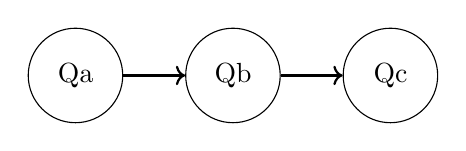
\begin{tikzpicture}[node distance=2cm, every node/.style={circle, draw, minimum size=1.2cm}]
  \node (Qa) {Qa};
  \node[right of=Qa] (Qb) {Qb};
  \node[right of=Qb] (Qc) {Qc};

  \draw[->, thick] (Qa) -- (Qb);
  \draw[->, thick] (Qb) -- (Qc);

\end{tikzpicture}
\caption{Connectivity of Three Qubits}
\label{fig:linearConnectivity}
\end{figure}
In this scenario, $\text{CNOT}_{a\rightarrow c}$ cannot be realized directly, it must be realized via qubit b:
\begin{equation}
    \text{CNOT}_{a\rightarrow c}=\text{CNOT}_{b\rightarrow c}\text{CNOT}_{a\rightarrow b}\text{CNOT}_{b\rightarrow c}\text{CNOT}_{a\rightarrow b}.
    \label{decomCNOT}
\end{equation}
As we can see, the decompostion of $\text{CNOT}_{a\rightarrow c}$ is necessary, since we want to change the target qubit c without changing the state of ancilla qubit, which is qubit b here. Actually we can let $\ket{abc}=\ket{110}$ as the initial value of those three qubits, and if we want to obtain $\ket{111}$ via $\text{CNOT}_{a\rightarrow c}$, then the decomposition in Eq.~\ref{decomCNOT} is the only way.

\subsubsection{The CZ gate}
Its matrix form is
\begin{equation}
    CZ=\begin{bmatrix}
        1&0&0&0\\
        0&1&0&0\\
        0&0&1&0\\
        0&0&0&-1
    \end{bmatrix},
\end{equation}
and its functionality is:
\begin{itemize}
    \item when the control qubit is $\ket{1}$, $Z$ gate is exerted to the target qubit, which means the phase is flipped.
    \item When the control qubit is $\ket{0}$, the target qubit does not change.
\end{itemize}

Both CZ and CNOT can cause entanglement, and both of them can convert to each other via Hadamard gate:
\begin{equation}
    CNOT_{c,t}=(I\otimes H)\cdot CZ_{c,t}\cdot(I\otimes H),
\end{equation}
which means we can obtain CNOT gate via CZ gate and Hadamard gate.


\subsection{The Qiskit}
\begin{itemize}
    \item In Qiskit, the \tcbox[inlinebox]{TwoLocal} or \tcbox[inlinebox]{EfficientSU2} are used to construct parameterized ansatz. 
    \item In Qiskit, all the simulation can be done via \tcbox[inlinebox]{AerSimulator} to realize testing and optimization.
\end{itemize}

\subsubsection{Collection of Qiskit Code}
\begin{lstlisting}[language=Python, caption=Circuit Measurement, frame=single, label={lst:CircuitMeasure}]
from qiskit.opflow import PauliSumOp
from qiskit import QuantumCircuit, Aer, execute

# 假设你要测 H = 0.7 * ZI + 0.6 * IZ - 0.9 * ZZ
H = PauliSumOp.from_list([('ZI', 0.7), ('IZ', 0.6), ('ZZ', -0.9)])

# ansatz 电路
qc = QuantumCircuit(2)
qc.ry(0.5, 0)
qc.cx(0, 1)

# 添加测量操作（可用 Estimator 接口更高效）
\end{lstlisting}

\begin{lstlisting}[language=Python, caption=Generating Hamilton, frame=single, label={lst:HamiltonGeneration}]
from qiskit_nature.second_q.drivers import PySCFDriver
from qiskit_nature.second_q.mappers import JordanWignerMapper
from qiskit_nature.second_q.problems import ElectronicStructureProblem

# 构建分子对象
driver = PySCFDriver(atom='H .0 .0 .0; H .0 .0 .74', basis='sto3g')
problem = ElectronicStructureProblem(driver)

# 得到费米子哈密顿量
second_q_op = problem.second_q_ops()['ElectronicEnergy']

# 使用 JW 映射
mapper = JordanWignerMapper()
qubit_op = mapper.map(second_q_op)

print(qubit_op)

\end{lstlisting}

\begin{figure}[ht]
\centering
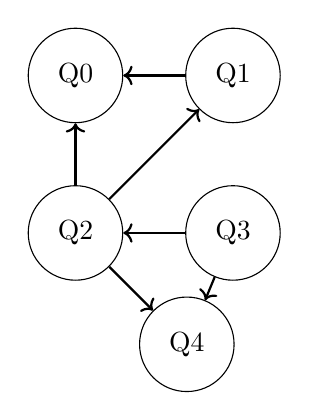
\begin{tikzpicture}[node distance=2cm, every node/.style={circle, draw, minimum size=1.2cm}]
  \node (Q0) {Q0};
  \node[right of=Q0] (Q1) {Q1};
  \node[below of=Q0] (Q2) {Q2};
  \node[below of=Q1] (Q3) {Q3};
  \node[below right of=Q2] (Q4) {Q4};

  \draw[->, thick] (Q1) -- (Q0);
  \draw[->, thick] (Q2) -- (Q0);
  \draw[->, thick] (Q2) -- (Q1);
  \draw[->, thick] (Q3) -- (Q2);
  \draw[->, thick] (Q3) -- (Q4);
  \draw[->, thick] (Q2) -- (Q4);
\end{tikzpicture}
\caption{Connectivity Graph of ibmqx4 Qubits}
\label{fig:connectivity}
\end{figure}
\section{Study of the Common Quantum Computing Algorithms}
\subsection{Grover's algorithm}
Grover's algorthim~\cite{Abhijith2018QuantumBeginner,NielsenChuang2010,Hidary2019QCBook} enables one to find a specific item within a randomly ordered database of $N$ using $O(\sqrt{N})$ operations. This approach can be used to accelerate the search by constructing an ``oracle'' which is in essence a quantum circuit that can flip the state of an ancillary qubit if the searching criterion is fullfilled. To this end, we need to set up a function $f(\boldsymbol{x})$ will output 1 if the input $\boldsymbol{x}$ equals the target value $\boldsymbol{x^*}$. Therefore, the functio is defined as
\begin{equation}
     f(\boldsymbol{x})=\begin{cases}
        1, & \qquad \text{if} \; \boldsymbol{x}=\boldsymbol{x^*} \\
        0, & \qquad \text{otherwise}
    \end{cases}.   
\end{equation}
With this function, we can turn any input into a binary output. For now, the function $f(\boldsymbol{x})$ is only an abstract symbole. Its specific form is decided by the problem we are solving. For example, if we want to find a naive result of $\boldsymbol{x^*}$ such that $x_1^*=1$ and $x_2^*=1$ for $\boldsymbol{x}=x_1x_2$. This essentially means $f(\boldsymbol{x})$ here is an AND gate. But AND is \textcolor{red}{not} reversible so that it cannot be a quantum gate. Fortunately, we have Toffoli gate which can take three bits as input and output three bits. The first two bits are used as the control bits so that the third bit flips if the control bits are all 1s. The details of the Toffoli can be found in section~\ref{sec:QuantumCircuit}. In other word, for this problem, the orcal quantum circuit can be realized by a Toffoli gate. In general, the functionality of the oracle is 
\begin{equation}
    \ket{\boldsymbol{x}}\ket{q}\overset{O} {\longrightarrow} \ket{\boldsymbol{x}}\ket{f(\boldsymbol{x})\oplus q}, 
\end{equation}
where $O$ is the oracle operator and $\oplus$ denots XOR operation. Based on the oracle opertor $O$, Grover operator is defined
\begin{equation}
    G=(2\ket{\psi}\bra{\psi}-I)O,
\end{equation}
where $\ket{\psi}=\frac{1}{\sqrt{N}}\sum_i\ket{i}$ is the uniform superpostion over all the basis states and $I$ is the identity operator. Since by now, we have already known the behavior of oracle opertor $O$, then we need to analyze the purpose of $(2\ket{\psi}\bra{\psi}-I)$. Let use this part of operator onto an arbitary state, given by $\sum_i a_i\ket{i}$. Please note the arbitary state is different from the $\ket{\psi}$ for the previous one does not have equal amplitude for each component. This is important, since the change of the amplitudes will become one of main concerns of this algorithm. Therefore,
\begin{equation}
    (2\ket{\psi}\bra{\psi}-I)\sum_i a_i\ket{i}=\sum_i(2\langle a\rangle-a_i)\ket{i}.
    \label{eqn:FlipMeanAmplitude}
\end{equation}
From the Eq.~\ref{eqn:FlipMeanAmplitude}, the effect of the operator on the arbitary state is to flip the amplitude of each component $\ket{i}$ (with the amplitude of $a_i$) about the mean amplitude $\langle a\rangle$. This property plays a very important role in this scheme. For this reason, a brief explanation over the expression $2\langle a\rangle-a_i$ is necessary. Suppose, without losing generality, $a_i>\langle a\rangle$, then the distance between the two value is $a_i-\langle a\rangle$. After flipping, the new value is $\langle a\rangle -(a_i-\langle a\rangle)$, hence the result $2\langle a\rangle-a_i$. 

Now, it is time to get the initial state ready as shown in the following figure (the first two are the input qubits and the third is the ancillary qubit):
\begin{figure}[ht]
\centering
    \begin{quantikz}
    \lstick{$\ket{0}$} & \gate{H} & \qw &\rstick[2]{\ket{\psi}} \\
    \lstick{$\ket{0}$} & \gate{H} & \qw &\\
    \lstick{$\ket{0}$} & \gate{X} & \gate{H} & \qw \rstick{\ket{-}}
    \end{quantikz}
\caption{State Preparation}
\label{fig:StatePreparation}
\end{figure}
After the Hadamard transformation, the two $\ket{0}$s are turned into $\ket{\psi}$ and the ancillary qubit is turned into $\frac{\ket{0}-\ket{1}}{\sqrt{2}}$. So, the prepared state is $\ket{\psi}\frac{\ket{0}-\ket{1}}{\sqrt{2}}$. If the input value is exactly what we are looking for, then the oracle operator will disclose
\begin{equation}
    O\ket{\boldsymbol{x^*}}\frac{\ket{0}-\ket{1}}{\sqrt{2}}\rightarrow\ket{\boldsymbol{x^*}}\frac{\ket{f(\boldsymbol{x^*})\oplus0}-\ket{f(\boldsymbol{x^*})\oplus1}}{\sqrt{2}}=\ket{\boldsymbol{x^*}}\frac{\ket{1}-\ket{0}}{\sqrt{2}}=-\ket{\boldsymbol{x^*}}\frac{\ket{0}-\ket{1}}{\sqrt{2}}.
    \label{eqn:FlipAmp}
\end{equation} 
From this equation we can see, if oracle operator is exerted on the target value $\ket{\boldsymbol{x^*}}$, its amplitude will be changed into its oppsite number, while other state will be the same. This will make a big difference between the targeted state and the other states, since the "flipped about the mean amplitude" will be followed. Then we can repeat this procedure many times and the difference will be accumulated until the target state is well-marked.  In the worst case, this procedure will be repeated for $\frac{\pi\sqrt{N}}{4}$ times.
\subsection{Bernstein-Vazirani Algorithm}
BV algorithm~\cite{Abhijith2018QuantumBeginner,NielsenChuang2010,Hidary2019QCBook} is used to solve this type of problems: suppose we have a classical Boolean function $f:\{0,1\}^n\mapsto\{0,1\}$. If there is a \textit{hidden string} $\textbf{s}$ which is unknow, this Boolean function can always be expressed as $f_\textbf{s}(\textbf{x})=\oplus_is_i x_i\equiv\langle\textbf{s},\textbf{x}\rangle$ which can be evaluated by an oracle like we saw in Grover's algorithm, then the question is can we find out the hidden string with just a single application of the oracle?

More note on $f:\{0,1\}^n\mapsto\{0,1\}$ and $f_\textbf{s}(\textbf{x})=\oplus_is_i x_i\equiv\langle\textbf{s},\textbf{x}\rangle$. Here $\{0,1\}^n$ means a set of binary string, and $n$ is the length of the string. For example, when $n=2$, this set contains elements like {(00), (01), (10), (11)}. As to the definition of $\langle\textbf{s},\textbf{x}\rangle$, we can understand it via a specific example. If we have $\textbf{s}=(1, 0, 1)$ and $\textbf{x}=(1, 1, 1)$, then the expansion of $\oplus_is_i x_i$ is $(1\times1+0\times1+1\times1) \; \text{mod}\; 2$. Two details need to be emphasized here: first, the \textcolor{red}{mod 2} is mandatory; second, the digit in the binary string is the \textbf{index} of qubit, not the component of the vector on that qubit. For example, our convention is like $\ket{0}=\begin{bmatrix}
    1\\0
\end{bmatrix}$. If you have a digital 0 at hand, then this 0 is the 0 on the left side of the equation, not the second component on the right side of the equation. 

Similar to Grover's algorithm, we need an oracle $U_s$ to evaluate the function $f_\textbf{s}(\textbf{x})$. Due to requirement of unitarity and reversiblity, the oracle operator also needs to work on an ancilla qubit $\ket{q}$~\cite{RobertLoredo2020}. Therefore, we have 
\begin{equation}
    U_s\ket{\textbf{x}}\ket{q}=\ket{\textbf{x}}\ket{q\oplus\langle\textbf{s},\textbf{x}\rangle}.
\end{equation}
Denoting $\ket{-}=(|0\rangle-|1\rangle)/\sqrt{2}$, we can verify from Eq.~\ref{eqn:FlipAmp} that,
\begin{equation}
    U_s|\textbf{x}\rangle|-\rangle=(-1)^{\langle\textbf{s},\textbf{x}\rangle}|\textbf{x}\rangle|-\rangle.
\end{equation}
Meanwhile, the \textit{n}-qubit Hadamard operator can be expanded in the outer-product form:
\begin{equation}
    H^{\otimes n}=\frac{1}{\sqrt{2^n}}\sum_{\textbf{x, y}\in\{0,1\}^n}(-1)^{\langle\textbf{x},\textbf{y}\rangle}\ket{\textbf{y}}\bra{\textbf{x}}
    \label{eqn:NqubitHadamard}
\end{equation}
$U_s$ and $H^{\oplus n}$ are the only two operators used in the BV algorithm, and the process is presented by
\begin{equation}
    \begin{split}
    \ket{0}^n\ket{n}\xrightarrow{H^{\otimes (n)}\otimes H} \frac{1}{\sqrt{2^n}}\sum_{\textbf{x}=0}^{2^n-1}\ket{\textbf{x}}\otimes\ket{-}\overset{U_s}{\rightarrow}\frac{1}{\sqrt{2^n}}\sum_{\textbf{x}=0}^{2^n-1}(-1)^{\langle\textbf{s},\textbf{x}\rangle}\ket{\textbf{x}}\otimes\ket{-}\\ 
    \overset{H^{\otimes n}}{\longrightarrow}\frac{1}{\sqrt{2^n}}\sum_{\textbf{x, y}=0}^{2^n-1}(-1)^{\langle\textbf{s},\textbf{x}\rangle\oplus\langle\textbf{x},\textbf{y}\rangle}\ket{y}\otimes\ket{-}\equiv\ket{\textbf{s}}\otimes\ket{-}.
    \end{split}
\end{equation}
\subsection{The Quantum Fourier Transform (QFT)}
QFT is a core quantum computing algorithm plays an important role in a couple of other algorithms~\cite{NielsenChuang2010}. QFT is based on the classical \textit{discrete Fourier Transform} (DFT), which takes as input a vector of complex numbers, $x_0,...,x_{N-1}$ where the length $N$ is a fixed parameter. The output of the DFT is another set of complex numbers $y_0,...,y_{N-1}$ which is related to the input $x$s by
\begin{equation}
    y_k\equiv\frac{1}{\sqrt{N}}\sum_{j=0}^{N-1}x_je^{2\pi ijk}/N.
\end{equation}
Its inverse is given by
\begin{equation}
    x_j\equiv\frac{1}{\sqrt{N}}\sum_{j=0}^{N-1}y_ke^{-2\pi ijk}/N.
\end{equation}
In QFT, DFT is done on the \textit{amplitude} of a quantum state
\begin{equation}
    \sum_{j=0}^{N-1}x_j\ket{j}\longrightarrow\sum_{k=0}^{N-1}y_k\ket{k},
\end{equation}
where, as we can see, the  $y_k$ are now the DFT of the amplitude of $x_j$. Such a transform is possible as long as we can find a unitary operator $\hat{F}$ such that
\begin{equation}
    \ket{\tilde{\psi}}=\hat{F}\ket{\psi}, \quad \text{with}\quad\hat{F}^\dagger\hat{F}=\hat{I}.
\end{equation}
Similar to Eqn.~\ref{eqn:NqubitHadamard}, both $\hat{F}^{\dagger}$ and $\hat{F}$ can be written into the outer product form:
\begin{equation}
    \hat{F}^\dagger=\left(\sum_{j,k}\frac{e^{-2xijk/N}}{\sqrt{N}}\ket{j}\bra{k}\right), \quad \text{and}\quad \hat{F}=\left(\sum_{j^{\prime},k^{\prime}}\frac{e^{2xij^{\prime} k^{\prime}/N}}{\sqrt{N}}\ket{k^{\prime}}\bra{j^{\prime}}\right).
\end{equation}
With this, it is easy to confirm that $\hat{F}^\dagger\hat{F}=\hat{I}$. 

Let $N=2^n$, where $n$ is the number of qubit. The basis $\ket{0}, ...,\ket{2^n-1}$ is the computational basis for those qubits. In other words, we have $\ket{j}$ with $0 \le j\le n-1$. Now, there comes the tricky part, in the upcoming discussion, instead of using decimal number $j$, we use its corresponding binary form $j_1j_2...j_n$ fulfills $j=j_12^{n-1}+j_22^{n-2}+\cdots+j_n2^0$. As for the \textit{binary fraction}, we have $j_l/2+j_{l+1}/4+\cdots+j_m/2^{m-l+1}$, we use the notation $0.j_lj_{l+1}\cdots j_m$. With these notations, the transformation
\begin{equation}
    \ket{j}\longrightarrow\frac{1}{\sqrt{N}}\sum_{k=0}^{N-1}e^{2\pi ijk/N}\ket{k}.
    \label{eqn:basisTransfrom}
\end{equation}
\begin{example}
    For $\ket{0}$, we have
    \begin{equation}
        \ket{0}\rightarrow\frac{1}{\sqrt{N}}\sum_{k=0}^{N-1}e^{2\pi i 0 k/N}\ket{k}.
        \label{eqn:QFTof0}
    \end{equation}
    Since $k$ is a binary number, which means $k\in \{0,1\}$, then $N=2$. Eqn. (\ref{eqn:QFTof0}) can be further expanded into $\frac{1}{\sqrt{2}}(\ket{0}+\ket{1})$. Based on that, it is easy to see
    \begin{equation}
        \begin{split}
            \ket{00}=\ket{0}\ket{0}&\rightarrow\frac{1}{2}(\ket{0}+\ket{1})\otimes(\ket{0}+\ket{1}) \\
            &=\frac{1}{2}(\ket{00}+\ket{10}+\ket{01}+\ket{11}).
        \end{split}
    \end{equation}
    So, the Fourier transform of the $n$ qubit state $\ket{00...0}$ is $\frac{1}{2^{n/2}}\left(\ket{00...0}+\ket{10...0}+\cdots+\ket{11...1}\right)$
    \label{exp:QFT1}
\end{example}
Follow the idea of Example \ref{exp:QFT1}, Eqn. \ref{eqn:basisTransfrom} can be written into the useful \textit{product representation}:
\begin{equation}
    \begin{split}
        &\ket{j_1,\cdots,j_n}\rightarrow\\
        &\frac{1}{2^{n/2}}\left(\ket{0}+e^{2\pi i0.j_n}\ket{1}\right)\otimes\left(\ket{0}+e^{2\pi i0.j_{n-1}j_n}\ket{1}\right)\otimes\cdots\otimes\left(\ket{0}+e^{2\pi i0.j_1j_2\cdots j_n}\ket{1}\right).
    \end{split}   
   \label{eqn:ProductRepre}
\end{equation}
The equivalence between Eqn.~\ref{eqn:basisTransfrom} and Eqn.~\ref{eqn:ProductRepre} can be mathematically proved by
\begin{equation}
    \begin{split}
        \ket{j}&\rightarrow\frac{1}{2^{n/2}}\sum_{k=0}^{2^n-1}e^{2\pi ijk/2^{n}}\ket{k}\\
        &=\frac{1}{2^{n/2}}\sum_{k_1=0}^1\cdots\sum_{k_n=0}^1e^{2\pi ij(\sum_{l=1}^nk_l2^{-l})}\ket{k}\\
        &=\frac{1}{2^{n/2}}\sum_{k_1=0}^1\cdots\sum_{k_n=0}^1\bigotimes_{l=1}^ne^{2\pi ijk_l2^{-l}}\ket{k_l}\\
        &=\frac{1}{2^{n/2}}\bigotimes_{l=1}^n\left[\sum_{k_l=0}^1e^{2\pi ijk_l2^{-l}}\ket{k_l}\right]\\
        &=\frac{1}{2^{n/2}}\bigotimes_{l=1}^n\left[\ket{0}+e^{2\pi ij2^{-l}}\ket{1}\right].
    \end{split} 
    \label{eqn:ProveEquivalence}
\end{equation}
It is easy to see, the last line of Eqn.~\ref{eqn:ProveEquivalence} is equivalent to the right side of Eqn.~\ref{eqn:ProductRepre}. Now, we can see the significance of Eqn.~\ref{eqn:ProductRepre} lies in the fact that the unitary 
\begin{equation}
    \ket{0,1}\longrightarrow\frac{1}{\sqrt{2}}(\ket{0}\pm e^{i\theta}\ket{1})
\end{equation}
is a Hadamard gate followed by a $Z$-rotation by $\theta$ defined by
\begin{equation}
    Z(\theta)=\begin{bmatrix}
        1&0\\
        0&e^{i\theta}
    \end{bmatrix}
\end{equation}
In Eqn.~\ref{eqn:ProductRepre}, the rotation depends on the values of the other bits. So we should expect to be able to build the QFT out of \textit{Hadamards} and \textit{controlled-phase rotation gates}. Define the rotation
\begin{equation}
    \hat{R}_k=\begin{bmatrix}
        1&0\\
        0&e^{2\pi i/2^k}
    \end{bmatrix}.
\end{equation}
The controlled-$\hat{R}_k$ gate performs if and only if a control bit is $\ket{1}$ rather than $\ket{0}$. Putting those together, we can get figure~\ref{fig:QFT}. In the first line of this figure, after applying the Hadamard gate to the first bit produces the state
\begin{equation}
    \frac{1}{\sqrt{2}}\left(\ket{0}+e^{2\pi i0.j_1}\right)\ket{j_2,\cdots,j_n}.
\end{equation}
This process continues for the rest of the qubit, giving the final state
\begin{equation}
    \frac{1}{2^{n/2}}\left(\ket{0}+e^{2\pi i0.j_1j_2\cdots j_n}\ket{1}\right)\otimes\left(\ket{0}+e^{i\pi i0.j_2\cdots j_n}\ket{1}\right)\otimes\cdots\otimes\left(\ket{0}+e^{2\pi i0.j_n}\right).
    \label{Eqn:AfterQTFFigure}
\end{equation}
Compare Eqn.~\ref{Eqn:AfterQTFFigure} and Eqn.~\ref{eqn:ProductRepre}, we can see swap operations are needed to reach the desired result. Therefore, it is time for us to count the total number of the gates needed in this circuit. For the first qubit, there are one Hadamard gate and $n-1$ conditional rotation -- a total of $n$ gates. Then, for the second qubit, one Hadmard gate plus $n-2$ conditional rotations leads to $n-1$ gates. So we need $n+(n-1)$ gates for the first two qubits. This counting proceeds for the rest ends up with $n(n+1)/2$ total number of gates. Don't forget we also need to take into account $n/2$ swaps, each of which need three controlled-NOT gates. Therefore, this circuit provides a $\Theta(n^2)$ algorithm for pefroming the quantum Fourier Transform. Compared to the best classical algorithm for \textit{Fast Fourier Transform} (FFT) requirement of $\Theta(n2^n)$, the quantum computing is terrific. However, it is still unknown for now whether the QFT can be used to real problem directly to speed up the computation as commemnted in~\cite{NielsenChuang2010}.
\begin{quote}
    \ttfamily
    \raggedright
    \enquote{The problem is that the amplitude in a quantum computer cannot be directly accessed by measurement. Thus, there is no way of determining the Fourier transfomed amplitudes of the original state. Worse still, there is in general no way to efficiently prepare the original state to be Fourier transfomed. Thus, finding uses for the QFT is more subtle than we might have hoped.}
\end{quote}

\begin{figure}
    \centering
    \resizebox{\textwidth}{!}{
        \begin{quantikz}
            \lstick{$\ket{j_1}$} & \gate{H} & \gate{R_2} & \cdots & \gate{R_{n-1}} & \gate{R_n} &&&&&& \qw & \rstick{$\ket{0} + e^{2\pi i0.j_1\ldots j_n} \ket{1}$}\\
            \lstick{$\ket{j_2}$}&&\ctrl{-1}&\cdots&&&\gate{H}&\cdots&\gate{R_{n-2}}&\gate{R_{n-1}}& \cdots&\qw&\rstick{$\ket{0} + e^{2\pi i0.j_2\ldots j_n} \ket{1}$}\\
            \quad\vdots\qquad\qquad\vdots\\
            \lstick{\ket{j_{n-1}}}&&&&\ctrl{-3}&&&&\ctrl{-2}&\cdots&\gate{H}&\gate{R_2}&\rstick{$\ket{0} + e^{2\pi i0.j_{n-1}\ldots j_n} \ket{1}$}\\
            \lstick{\ket{j_n}}&&&&&\ctrl{-4}&&&&\ctrl{-3}&\cdots&\ctrl{-1}&\rstick{$\ket{0} + e^{2\pi i0.j_n} \ket{1}$}
        \end{quantikz}
    }
    \caption{Circuit of Quantum Fourier Transform}
    \label{fig:QFT}
\end{figure}

\subsection{Phase Estimation}
Phase Estimation (PE)~\cite{Abhijith2018QuantumBeginner,NielsenChuang2010} is one of the scenarios that the QFT can be used, and PE itself, as a quantum algorithm, can serve as a subroutine of other quantum computing application. PE is designed for solving a certain type of eigenvalue problem where a unitary operator $U$ has an eigenvector $\ket{u}$ with eigenvalue $e^{2\pi i\varphi}$, with unknown value of the $\varphi$.

To establish a complete PE, we first need an oracle (black box) to help us to prepare the state $\ket{u}$ and performing the controlled $U^{2^j}$ operation, where $j$ is a non-negative integer. After that, PE needs two type of register. One contains $t$ qubits initially in the state $\ket{0}$, the other is used to store $\ket{u}$. Based on the established hardware, PE can perform the following three steps:
\begin{enumerate}
    \item Circuit shown in Fig~\ref{fig:FirstStagePE} will be applied;
    \item \textit{Inverse} QFT will be performed on the first register;
    \item Read out the state of the first register by doing a measurement in the computational basis.
\end{enumerate}
% First stage of the PE
\begin{figure}
    \centering
    \resizebox{\textwidth}{!}{
        \begin{quantikz}
            \ \ \\
            \lstick[7]{First register \\ $t$ qubits} \ \ \\ \\  \\  \\  \\ \\[1.5cm]
            \ \ \\
            \ \ \\
            \lstick[2]{Second register}  \\ \\ \\
        \end{quantikz}
        \begin{quantikz}
            \lstick{$\ket{0}$} & \gate{H} &&&&\ \ldots\ & \ctrl{5} &  \qw &\ \ \rstick{$\ket{0} \quad e^{2\pi i(2^{t-1}\varphi)\ket{1}}$}\\
            \ \vdots \ \\
            \lstick{$\ket{0}$} & \gate{H} & & & \ctrl{3} &\ \ldots\ & \qw & \qw &\ \ \rstick{$\ket{0} \quad e^{2\pi i(2^{2}\varphi)\ket{1}}$} \\
            \lstick{$\ket{0}$} & \gate{H} & & \ctrl{2} & &\ \ldots\ & \qw & &\ \ \rstick{$\ket{0} \quad e^{2\pi i(2^{1}\varphi)\ket{1}}$} \\
            \lstick{$\ket{0}$} & \gate{H} &\ctrl{1} & \qw &\qw &\ \ldots\ &   & \qw &\ \ \rstick{$\ket{0} \quad e^{2\pi i(2^{0}\varphi)\ket{1}}$}\\
            \lstick[3, brackets=none]{$\ket{u}$}&  & \gate{U^{2^0}} & \gate{U^{2^1}} & \gate{U^{2^2}} &\ \ldots\ &\gate{U^{2^{t-1}}}&\qw& \rstick[3, brackets=none]{$\ket{u}$}
        \end{quantikz}
    }
    \caption{The First Stage of PE}
    \label{fig:FirstStagePE}
\end{figure}
As we can see in Fig.~\ref{fig:FirstStagePE}, this circuit starts by applying the Hadamard on the first register and then followed by application of controlled-$U$ operators on the second register. The result of this circuit is
\begin{equation}
    \frac{1}{2^{t/2}}\left(\ket{0}+e^{2\pi i2^{t-1}\varphi}\ket{1}\right)\otimes\left(\ket{0}+e^{2\pi i2^{t-2}\varphi}\ket{1}\right)\cdots\left(\ket{0}+e^{2\pi i2^0\varphi}\right)=\frac{1}{2^{t/2}}\sum_{k=0}^{2^t-1}e^{2\pi i\varphi k}\ket{k}.
    \label{eqn:AfterFirstRegister}
\end{equation}
If we expand $\varphi$ into its $t$ binary bit form and use the notation $\varphi=0.\varphi_1\cdots\varphi_t$, the left side of Eqn.~\ref{eqn:AfterFirstRegister} can be rewritten into
\begin{equation}
    \frac{1}{2^{t/2}}\left(\ket{0}+e^{2\pi i0.\varphi_1}\ket{1}\right)\otimes\left(\ket{0}+e^{2\pi i0.\varphi_{t-1}\varphi_t}\ket{1}\right)\cdots\left(\ket{0}+e^{2\pi i0.\varphi_1\varphi_2\cdots\varphi_t}\ket{1}\right),
\end{equation}
which is exactly the same as Eqn.~(\ref{eqn:ProductRepre}). Therefore, the second step of PE is to apply the inverse QFT, which gives rise to the product state $\ket{\varphi_1\cdots\varphi_t}$. The measurement will tell us the exact value of $\varphi$. This is an ideal scenario when $\varphi$ can be expressed as a $t$ bit binary expansion. However, even if this condition is not fully fullfilled, it turns out that the procedure will produce a pretty good approximation with high probability.

\subsection{HHL Algorithm for Linear Systems Problem}
Linear system problem can be met everywhere. To solve it on a quantum computer, we need to make use of the QFT and PE analyzed above. This problem is defined as
\begin{equation}
    A\ket{x}=\ket{b},
\end{equation}
where $A$ is a Hermitian matrix and both solution to be found $\ket{x}$ and the constant vector $\ket{b}$ have already been normalized, which means $\left\|\vec{x}\right\|=\left\|\vec{b}\right\| =1$. The solution can be expressed as $\ket{x}=\frac{A^{-1}\ket{b}}{\left\| A^{-1}\ket{b}\right\| }$. When $\left\| A^{-1}\ket{b}\right\|=1$, this expression can be further simplified as
\begin{equation}
    \ket{x}=A^{-1}\ket{b}
    \label{eqn:solutionofA}
\end{equation}

The quantum algorithm  for the linear system was first proposeb by Harrow, Hassidim, and Lloyd, and hence the short name HHL. Mathematical formulation can be summarized briefly below.
Using spectral decompostion theorem, operator $A$ can be expressed as 
\begin{equation}
    A=\sum_{j=0}^{N-1}\lambda_j\ket{u_j}\bra{u_j},
    \label{eqn:SpectralDecomposition}
\end{equation}
where $\lambda_j$ is the $j^{\text{th}}$ eigenvalue of matrix $A$. Since $A$ is Hermitian, its eigenvectors can form orthonormal basis, and its inverse can be expressed as
\begin{equation}
    A^{-1}=\sum_{j=0}^{N-1}\lambda_j^{-1}\ket{u_j}\bra{u_j}.
    \label{eqn:inverseofA}
\end{equation} 
Now, let's express the constant vector $\ket{b}$ in terms of eigenbasis of $A$:
\begin{equation}
    \ket{b}=\sum_{j=0}^{N-1}b_j\ket{u_j}.
\end{equation}
Together with Eqn.~\ref{eqn:solutionofA} and Eqn.~\ref{eqn:inverseofA}, we can see 
\begin{equation}
    \begin{split}
        \ket{x}&=\left(\sum_{j=0}^{N-1}\lambda_j^{-1}\ket{u_j}\bra{u_j}\right)\left(\sum_{i=0}^{N-1}b_i\ket{u_i}\right)\\
        &=\sum_{j=0}^{N-1}\sum_{i=0}^{N-1}\lambda_j^{-1}b_i\ket{u_j}\langle u_j|u_i\rangle \\
        &=\sum_{j=0}^{N-1}\lambda_j^{-1}b_j\ket{u_j}.
    \end{split}
    \label{eqn:expandX}
\end{equation}
It is apparent from the Eqn.~\ref{eqn:expandX} that if we want to figure out $\ket{x}$, we need to know the knowledge of the eigenvalues of $A$, which can be obtained from the PE algorithm above. Therefore, we have the circuit below to help us do the job.
\begin{figure}
    \centering
    \begin{quantikz}
        \lstick{$\ket{0}$} & \slice{$\ket{\psi_0}$} & \slice{$\ket{\psi_1}$} & \slice{$\ket{\psi_2}$} & \gate{\hat{R}}\slice{$\ket{\psi_3}$}&\meter{}& \qw & \rstick{$\ket{1}$} \\
        \lstick{$\ket{0}^{\otimes n_l}$} & \qwbundle{n_l} && \gate[2]{PE}&\ctrl{-1}&&\gate[2]{PE^\dagger}&\rstick{$\ket{0}$} \\
        \lstick{$\ket{0}^{\otimes n_b}$} & \qwbundle{n_b} & \gate{\hat{U}_b} & & & & & \rstick{$\ket{x}$}
    \end{quantikz}
    \caption{Circuit of HHL}
    \label{fig:HHL}
\end{figure}

\subsection{Sample-based Quantum Diagonalization of a Chemistry Hamiltonian}
Sample-based quantum diagonalization (SQD) algorithm \cite{Robledo_Moreno_2025, ibm2024sqd} is a method for finding eigenvalues and eigenvectors of quantum opertors, using quantum and distributed classical computing together. Classical distributed computing is used to process samples obtained from a quantum processor, and to project and diagonalize a target Hamiltonian in a subspace spanned by them. SQD is known to work well when the target eigenstate is sparse.

In \ref{sec:MappingMethods}, we have learned in quantum chemistry the formalism of second quantization can be used to describe the electronic structure of a molecule. Upon the definition of annihilation operator and creation operator, we also defined their anti-commutation relations in Eqn.~\ref{eqn:anti-comm}. However, in this construction, the spin, which is an important feature of electron, was not taken into account. To compensate that, we introduce lables $\hat{\alpha}_{p\sigma}$, where $\sigma$ is used to include either spin-up state $\alpha$ or spin-down state $\beta$. Accordingly, Eqn~\ref{eqn:secondQuantizedHam} is updated into
\begin{equation}
    \hat{H}=\sum_{pr\sigma}h_{pr}\hat{a}^{\dagger}_{p\sigma}\hat{a}_{r\sigma}+\frac{1}{2}\sum_{prqs\sigma\tau}h_{prqs}\hat{a}^{\dagger}_{p\sigma}\hat{a}^{\dagger}_{q\tau}\hat{a}_{s\tau}\hat{a}_{r\sigma},
\end{equation}
where again $h_{pr}$ and $h_{prqs}$ are complex numbers from molecular integrals.

\subsubsection{Unitary Cluster Jastrow (UCJ) ansatz}
SQD requires a quantum circuit ansatz to draw samples from Local UCJ (LUCJ) \cite{motta2023lucj}, due to its combination of physics and hardware friendliness, is adopted here. This ansatz is based on UCJ ~\cite{Jastrow1955} which was first proposed by Robert Jastrow to solve many-body problem with strong forces. To address the short range strong force problem, he introduced a product of  exponentialized wavefunctions containing a parameter that can be used in variational computation to reach the minimum energy of a quantum system. This wavefunction, which is later called unitary cluster Jastrow (UCJ), can fit into the current quantum computing to solve quantum chemistry problem. It looks like
\begin{equation}
    |\psi\rangle=\prod_{\mu=1}^{L}e^{\hat{K}_\mu}e^{i\hat{J}_\mu}e^{-\hat{K}_\mu}|\Phi_0\rangle,
    \label{eqn:UCJ}
\end{equation}
where $|\Phi_0\rangle$ is a reference state, often taken to be the Hartree-Fock state, and the $\hat{K}_\mu$ and $\hat{J}_\mu$ are defined as \cite{ibm2024sqd,motta2023lucj}
\begin{equation}
    \hat{K}_\mu=\sum_{pq,\sigma}K^\mu_{pq}\hat{a}^\dagger_{p\sigma}\hat{a}_{q\sigma}, \: \hat{J}_\mu=\sum_{pq,\sigma\tau}J_{pq,\sigma\tau}^\mu\hat{n}_{p\sigma}\hat{n}_{q\tau},
    \label{eqn:1-2-bodyOperator}
\end{equation}
where $\hat{n}_{p\sigma}=\hat{a}^\dagger_{p\sigma}\hat{a}_{p\sigma}$ is known as the number operator and $K_{pq}^\mu$ is the complex matrix elements forms an anti-Hermitian matrix, whereas $J_{pq,\sigma\tau}^\mu$ is real and it forms a symmetric matrix. To maintain the spin symmetry, $\hat{J}$ should commute with the z-component of the total spin operator $S_z=\frac{1}{2}\sum_p(\hat{n}_{p\alpha}-\hat{n}_{p\beta})$, which is in essence the weighted summation of particle number. Therefore, the conditions like
\begin{equation}
    J_{pq,\alpha\alpha}^\mu=J_{pq,\beta\beta}^\mu, \: J_{pq,\alpha\beta}^\mu=J_{pq,\beta\alpha}^\mu
\end{equation}
should be guaranteed. Meanwhile, note that commutation with $S^2$ operator requires $J_{pq,\alpha\alpha}^\mu=J_{pq,\alpha\beta}^\mu$, eqn (\ref{eqn:1-2-bodyOperator}) can be reorganized and written as
\begin{multline}
    \hat{J}_\mu=2\sum_pJ_{pp,\alpha\beta}^\mu\hat{n}_{p\alpha}\hat{n}_{p\beta}+4\sum_{p<q}J_{pq,\alpha\beta}^\mu\hat{n}_{p\alpha}\hat{n}_{q\beta}+2\sum_pJ_{pp,\alpha\alpha}^\mu[\hat{n}_{p\alpha}+\hat{n}_{p\beta}] \\
    +2\sum_{p<q}J_{pq,\alpha\alpha}^\mu[\hat{n}_{p\alpha}\hat{n}_{q\alpha}+\hat{n}_{p\beta}\hat{n}_{q\beta}]
    \label{eqn:rewriteJ}
\end{multline}
On the right of the eqn (\ref{eqn:rewriteJ}), the first term is on-site opposite-spin term; the second one is the non-diagonal opposite-spin term; the third term is the on-site same-spin term, and the last one is the non-diagonal same-spin term.

In eqn (\ref{eqn:UCJ}), the operator $e^{\hat{K}_\mu}$ is also regarded as the rotational operator over the orbitals whose function is to rotate the given basis to new basis. By doing so, the redistribution of the electrons within the orbitals is realized. In this process, the total number of electrons and their spin state are conserved. From the point of view of group theory, the unitary rotational operator $e^{\hat{K}_\mu}$ is a Lie group element while the operator $\hat{K}_\mu$ as its Lie algebra generator. In practice, such a rotation is realized on the quantum computing circuit via a serise of Givens rotation which will be disscussed in details later. In contrast, the number-number interaction operator $\hat{J}_\mu$ realizes the modulation of electron correlation. Therefore, unlike $\hat{K}_\mu$， it is a two-body operator. The sandwitch shape structure $e^{\hat{K}_\mu}e^{i\hat{J}_\mu}e^{-\hat{K}_\mu}$ composed of those two types of operators is a similarity transformatioFn. When it is applied onto a reference state like we saw in eqn (\ref{eqn:UCJ}), it implies three steps. First, it rotates reference state $|\psi_0\rangle$ into new orbital basis via $e^{-\hat{K}_\mu}$, then $e^{i\hat{J}_\mu}$ will exert electron correlation modulation on the new basis, i.e. the Jastrow factor. After that, it will change the basis back via $e^{\hat{K}_\mu}$.

Now, suppose we are going to use the widely used JW mapping scheme (see section \ref{sec:MappingMethods}), $N$ spatial orbitals should be mapped onto a system of $2N$ qubits,
\begin{equation}
    \hat{a}^\dagger_{p\alpha}\mapsto(S_+)_p Z_{(p-1)}... Z_0, \: \hat{a}^\dagger_{p\beta}\mapsto(S_+)_{N+p} Z_{N+p-1}...Z_0,
\end{equation}
where $(S_+)_p=(X_p+iY_p)/2$ is the raising operator for qubit $p$. From here we can see, to achieve linear connectivity, we need $\mathcal{O}(N^2)$ Givens rotations acting on adjacent qubits. Considering eqn (\ref{eqn:rewriteJ}), the operator $e^{i\hat{J}_\mu}$ is mapped onto a quantum circuit of the form
\begin{equation}
    \begin{split}
        e^{i\hat{J}_\mu}&\mapsto\prod_p v_{p,p+N}(2J_{pp,\alpha\beta}^\mu)\prod_{p<q}v_{p,q+N}(4J_{pq,\alpha\beta}^\mu)\prod_{p}w_p(2J_{pp,\alpha\alpha}^\mu)w_{p+N}(2J_{pp,\alpha\alpha}^\mu) \\
    &\times\prod_{p<q}(2J_{pq,\alpha\beta}^\mu)v_{p+N,q+N}(2J_{pq,\alpha\beta}^\mu),
    \end{split}   
    \label{eqn:mapofJmu} 
\end{equation}
where $w_p(\phi)=e^{-i\frac{\phi}{4}Z_p}$ is a single-qubit gate and
\begin{equation}
    v_{p,q}(\phi)=e^{-i\frac{\phi}{4}(Z_p+Z_q-Z_pZ_q)}
\end{equation}
is a two-qubit gate. Eqn (\ref{eqn:mapofJmu}) indicates that we need $\mathcal{O}(N^2)$ two-qubit gates with all-to-all connectivity. In summary, we can say the UCJ is not applicabale to current hardware.
\subsubsection{Local Unitary Cluster Jastrow (LUCJ)}
To overcome the problem of UCJ addressed in the previous subsection, we introduce ``local'' approximation of the UCJ ansatz, which needs the following modifications for opposite-spin and same-spin number-number terms:
\begin{equation}
    \sum_{pq}J_{p\alpha,q\beta}\hat{n}_{p\alpha}\hat{n}_{p\beta}\rightarrow\sum_pJ_{p\alpha,p\beta}\hat{n}_{p\alpha}\hat{n}_{p\beta}
    \label{eqn:sparse1}
\end{equation}
\begin{equation}
    \sum_{pq}J_{p\sigma,q\sigma}\hat{n}_{p\sigma}\hat{n}_{q\sigma}\rightarrow\sum_pJ_{p\sigma,(p+1)\sigma}\hat{n}_{p\sigma}\hat{n}_{(p+1)\sigma},\:\text{where}\:\sigma=\alpha,\beta
    \label{eqn:sparse2}
\end{equation}
From the two equations above, we can see the summation over $p$ and $q$ is simplified into summation of $p$ only. By doing so, we neglect all the terms with $p\neq q$ so that only diagonal double occupation penalty terms are kept for opposite-spin terms. As for the same-spin term, the summation is performed over neigboring terms. Obviously, this approximation only takes into account the strongest electronic repulsion. In other words, two sparse matrices with the elements of $J_{p\alpha,q\alpha}^\mu$ and $J_{p\alpha,q\beta}^\mu$ respectively are formed. This allows us to implement the circuit in a constant depth with limited connectivity. For example, if the connectivity is a square lattice show in the figure \ref{fig:SquareCon}.
\begin{figure}
    \centering
    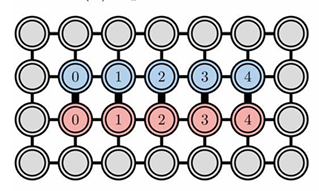
\includegraphics[width=0.3\textwidth]{square_connect.png}
    \caption{Square Connectivity}
    \label{fig:SquareCon}
\end{figure}
 In vector form, the summation corresponding to eqns (\ref{eqn:sparse1}, \ref{eqn:sparse2})
\begin{equation}
    \begin{split}
        &\boldsymbol{J}^{\alpha\alpha}:\{(p,p+1), p=0,...,N-2\} \\
        &\boldsymbol{J}^{\alpha\beta}:\{(p,p),p=0,...,N-1\}
    \end{split}
\end{equation} 
 Similarly, in the case of the heavy-hex lattice (see fig \ref{fig:heavyHex}), the sparse matrices are
 \begin{equation}
    \begin{split}
        &\boldsymbol{J}^{\alpha\alpha}:\{(p,p+1), p=0,...,N-2\} \\
        &\boldsymbol{J}^{\alpha\beta}:\{(p,p),p=0,4,8,...(p\leq N-1)\}
    \end{split}
 \end{equation}
 \begin{figure}
    \centering
    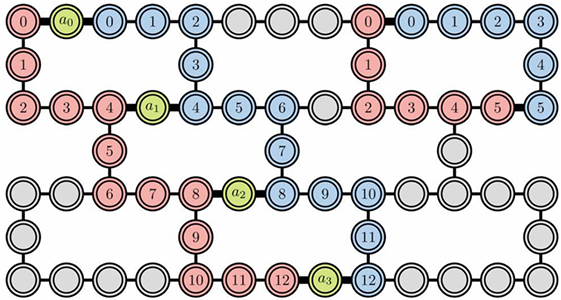
\includegraphics[width=0.4\textwidth]{heavy_hex.png}
    \caption{Heavy-hex lattice}
    \label{fig:heavyHex}
 \end{figure}

\section{Paper-reading related to adaptive grid method}
In the paper \textit{Real-Space Chemistry on Quantum Computers: A Fault-Tolerant Algorithm with Adaptive Grids and Transcorrelated Extension} \cite{feniou2025realspacechemistryquantumcomputers}, an adaptive grid method for quantum chemistry presented in the form of first-quantized real-space formulation is given. The following subsections are about my investigation of this paper and the collection of my understanding related to the topics contained in this paper.
\subsection{Voronoi Diagrams and Discretization of Wavefunction}
This subsection is dedicated the understanding of Eqn. (13) in this paper, which is about the discretization of a single electron wavefunction onto a multi-center grid with $N$ points, and it looks like
\begin{equation}
    \ket{\psi_e}=\sum_{m=0}^{N-1}c_m\ket{m},
    \label{eqn:discretizedBase}
\end{equation}
where $m$ runs through the indices of the cells in the Voronoi diagram.

To understand this formula correctly, the word ``discretization" is the key. Using Voronoi diagram, we have divided the 3D space into $N$ non-overlapping cells. Each cell corresponds to a grid point.  Since $\ket{m}$ is a discretized base, it means although the base is defined on the whole 3D space, it concentrates on the corresponding $m$th Voronoi cell with complex amplitude $c_m$ which fulfils $\sum_{m=0}^{N-1}|c_m|^2=1$. That means on the Voronoi cell $Vor(m)$, value of $\ket{m}$ is 1, and zero anywhere else. Therefore, unlike the continuous wavefunction, we do not need to consider the continuous boundary condition between each Voronoi cells. In the Hilbert space, the basis $\ket{m}$ forms an orthonormal basis which fulfils
\begin{equation}
    \bra{m^{\prime}}m\rangle=\delta_{m^{\prime}m}.
\end{equation}
\begin{example}
    Suppose we have divided the whole space into three Voronoi cells, corresponding to three basis: $\ket{0}=(1,0,0), \ket{1}=(0,1,0)$ and $\ket{2}=(0,0,1)$. Then the wavefunction can be written into
    \begin{equation}
        \ket{\psi}=c_0\ket{0}+c_1\ket{1}+c_2\ket{2}=(c_0,c_1,c_2).
    \end{equation}
    The scenario discussed above is for a single electron. If we have two electrons, each of them has 3 cells, then the dimensionality of the whole Hilbet space is $3\times 3=9$, and the wavefunction can be expressed as
    \begin{equation}
        \ket{\Psi}=\sum_{n,n=0}^{2}c_{mn}\ket{m}_1\otimes\ket{n}_2,
    \end{equation}
    which is mentioned later in the paper the tensor product of $\eta$ single-electron wavefunctions that lives in $\mathcal{H}_{\text{tot}}=\bigotimes_{i=1}^{\eta}\mathcal{H}_e$.
\end{example}

\subsection{Pauli decomposition}
\subsubsection{Equation 22}
 In order to understand the equation (22) in this paper, which looks like
\begin{equation}
    \bar{\textbf{H}}=\sum_{n,n=0}^{N-1}\omega_{mn}\sum_{i=0}^{\eta-1}\prod_{b=0}^{\log N - 1}\textbf{X}_{i\log N+b}^{m_b}\textbf{Z}_{i\log N+b}^{n_b}+\frac{1}{2}\sum_{m,p=0}^{N-1}\gamma_{mp}\sum_{i\neq j}^{\eta-1}\prod_{b=0}^{\log N-1}\textbf{Z}_{i \log N+b}^{m_b}\textbf{Z}_{j \log N+b}^{p_b},
\end{equation}
we track down to the paper \textit{Pauli Decomposition via the Fast Walsh-Hadamard Transform}\cite{Georges_2025}, which is a paper descibing the Pauli Linear Combination of Unitaries (LCU) decomposition.

Within the paper \cite{Georges_2025}, the collection of the Pauli matrices (see Table \ref{tab:gates}), are included in a set $\mathscr{P} \coloneqq \{I, X, Y, Z\}$. Based on that, a set  $\mathscr{P}_n$ of the dimension  $\mathbb{C}^{2n\times2n}$ is defined by
\begin{equation}
    \mathscr{P}_n \coloneqq \left\{\bigotimes_{j=0}^{n-1}P_j\,:\,P_j\in\mathscr{P}\right\}
\end{equation}
where $n$ is an integer. Then any complex matrix $A\in\mathbb{C}^{2n\times2n}$ can be expanded into a weighted sum of tensor products as
\begin{equation}
A=\sum_{P\in\mathscr{P}}\alpha(P)P,
\end{equation}
where the mapping $\alpha\coloneqq\mathscr{P}_n\rightarrow\mathbb{C}$ is called the Pauli coefficient which is theoretically given by
\begin{equation}
    \alpha(P)=\frac{1}{2^n}\text{tr}(A^\dagger P) \;\text{where}\; P\in\mathscr{P}_n.
    \label{eqn:PauliCoef}
\end{equation}
The problem to be addressed here is to compute the Pauli coefficients efficiently, since direct computation over Eqn~(\ref{eqn:PauliCoef}) has the scaling of  $\mathcal{O}(2^{5n})$. Plus, this equation is NOT easy to be used for LCU of a Hamiltonian or a matrix used in specific applications.

To overcome the difficulty, the authors of paper \cite{Georges_2025} proved the following theorem first. This theorem is expressed as:
\begin{theorem}
    (Pauli decomposition of $A\in\mathbb{C}^{2n\times2n}$ via the Walsh-Hadamard transfrom). The following decomposition
    \begin{equation}
        A=\sum_{r,s=0}^{2^n-1}\alpha_{r,s}P_{r,s},
    \end{equation}
    where
    \begin{equation}
        P_{r,s}\coloneqq\bigotimes_{j=0}^{n-1}(i^{r_j\wedge s_j}X^{r_j}Z^{s_j})\in\mathscr{P}_n\quad(r,s\in[2^n-1]_0)
    \end{equation}
    and
    \begin{equation}
        \alpha_{r,s}\coloneqq\frac{i^{-|r\wedge s|}}{2^n}\sum_{q=0}^{2^n-1}a_{q\oplus r,q}{(H^{\otimes n})_{q,s}}\quad(r,s\in[2^n-1]_0)
    \end{equation}
    holds. Conversly, ``A'' can be recovered from its Pauli string decomposition according to 
    \begin{equation}
        \alpha_{r,s}=i^{|\bar{r}\wedge s|}\sum_{q=0}^{2^n-1}\alpha_{r\oplus s, q}(H^{\oplus n})_{q,s}.
    \end{equation}
    \label{theo:PauliDecomp}
\end{theorem}
In Theorem(\ref{theo:PauliDecomp}), the symboles $\wedge, \oplus$ and $\bar{.}$ are the bitwise AND, XOR, and NOT operators. The symbole $|\cdot|$ denotes the Hamming weight.  For a given integer $N$, we define $[N]_0\coloneqq\{0,1,\dots,N\}$. Therefore, 
\begin{equation}
    [2^n-1]_0\coloneqq\{0,1,\dots,2^n-1\}.
    \label{eqn:numSet}
\end{equation} 
$r_j$ and $s_j$ are the binary expansion coefficients of $r$ and $s$, respectively. For the purpose of convenient reference, the well-known binary expansion for an integer $p$ is given as
\begin{equation}
    p=\sum_{j=0}^{n-1}p_j 2^j \quad (p_j\in\{0,1\})
\end{equation}
which defines a map $p\mapsto(p_j)_{j=0}^{n-1}\in\{0,1\}^n$. The bitwise XOR and AND are defined according to
\begin{equation}
    \text{XOR}: p\oplus q\coloneqq\sum_{j=0}^{n-1}(p_j\oplus q_j)2^j, \quad \text{AND}:p\wedge q\coloneqq\sum_{j=0}^{n-1}(p_j\wedge q_j)2^j\quad(p,q\in[2^n-1]_0).
    \label{eqn:bitwiseOperator}
\end{equation}
The Hamming weight is calculated according to
\begin{equation}
    |p|\coloneqq\sum_{j=0}^{n-1}p_j\quad(p\in[2^n-1]_0).
    \label{eqn:Hamming}
\end{equation}
\begin{example}
    Suppose we are studying a system of 3 qubits, which means $n=3$. According to Eqn. (\ref{eqn:numSet}), the number set we are dealing with is $\{0, 1, \dots, 7\}$. Let $p=6$ and $q=7$, we can easily see their binary forms are $p=6_{10}=110_2$ and $q=7_{10}=111_2$, respectively. Now, by making use of Eqn. (\ref{eqn:bitwiseOperator}), we can find the results of bitwise operator between $p$ and $q$. For XOR, it is $p\oplus q=6\oplus7=(0\oplus1)2^0+(1\oplus1)2^1+(1\oplus1)2^2=1$. For AND, it is $p\wedge q=6\wedge7=(0\wedge1)2^0+(1\wedge1)2^1+(1\wedge1)2^2=6$. Of course, for Hamming weight, for $p=6$, it is 0+1+1=2
    \label{exp:6.1}
\end{example}
Define a matrix unit for $\mathbb{C}^{2n\times2n}$ $E_{p,q}$ as
\begin{equation}
    E_{p,q}\coloneqq(\delta_{j,p}\delta_{k,q})_{j,k=0}^{2^n-1}\quad(p,q\in[2^n-1]_0),
    \label{eqn:MatrixUnit}
\end{equation}
which can also be written in the form
\begin{equation}
    E_{p,q}=\bigotimes_{j=0}^{n-1}e_j(p,q),
    \label{eqn:ExpandE}
\end{equation}
where
\begin{equation}
    e_j(p,q)\coloneqq(\delta_{k,p_j}\delta_{l,q_j})_{k,l=0}^1 \quad (j\in[n-1]_0;p,q\in[2^n-1]_0).
    \label{eqn:Define_e}
\end{equation}
Once again, those three equations can be checked by using a special scenario such that $n=3, p=6$ and $q=7$. According to Eqn (\ref{eqn:Define_e}), we will obtain an 8*8 matrix in which only the element in row 7 and column 8 is 1 and the rest elements are all zeros. This 8*8 matrix can be expanded into $\begin{bmatrix}
    0&0\\0&1
\end{bmatrix}\otimes\begin{bmatrix}
    0&0\\0&1
\end{bmatrix}\otimes\begin{bmatrix}
    0&1\\0&0
\end{bmatrix}$, which confirms the Eqn. (\ref{eqn:ExpandE}) and Eqn. (\ref{eqn:Define_e}).
Using the Pauli matrices as the basis, Eqn. (\ref{eqn:Define_e}) can be written into
\begin{equation}
    e_j(p,q)=\frac{1}{2}(X^{p_j\oplus q_j}+(-1)^{p_j}(iY)^{p_j\oplus q_j}Z^{\overline{p_j \oplus q_j}}).
\end{equation}
Considering $XZ=-iY$, Eqn. (\ref{eqn:ExpandE}) can be modified into
\begin{equation}
    \begin{split}
        E_{p,q}&=\frac{1}{2^n}\bigotimes_{j=0}^{n-1}(X^{p_j\oplus q_j}+(-1)^{q_j}X^{p_j\oplus q_j}Z) \\
        &=\frac{1}{2^n}\bigotimes_{j=0}^{n-1}\sum_{s_j=0,1}(-1)^{q_j\wedge s_j}X^{p_j\oplus q_j}Z^{s_j}\\
        &=\frac{1}{2^n}\prod_{j=0}^{n-1}\sum_{s_j=0,1}(-1)^{q_j\wedge s_j}X_j^{p_j\oplus q_j}Z_j^{s_j},
    \end{split}
    \label{eqn:DecompositionOfE}
\end{equation}
with 
\begin{equation}
    X_j\coloneqq I^{\otimes j}\otimes X\otimes I^{\otimes(n-j-1)}, \quad Z_j\coloneqq I^{\otimes j}\otimes Z\otimes I^{\otimes(n-j-1)}\quad (j\in[n-1]_0).
    \label{eqn:XandZ}
\end{equation}
The last step of Eqn. (\ref{eqn:DecompositionOfE}) makes sense because the operator $(-1)^{q_j\wedge s_j}X^{p_j\oplus q_j}Z^{s_j}$ only exert on the $j^{th}$ qubit, and with the definition from Eqn. (\ref{eqn:XandZ}) the last expression in Eqn. (\ref{eqn:DecompositionOfE}) will do the same job. Switching the sequence of the summation and production, the last expression can be written as
\begin{equation}
    E_{p,q}=\frac{1}{2^n}\left(\sum_{s_0=0,1}\cdots\sum_{s_{n-1}=0,1}\right)\prod_{j=0}^{n-1}(-1)^{q_j\wedge s_j}X^{p_j\oplus q_j}Z^{s_j}
    \label{eqn:Epq3}
\end{equation}
By transforming the $E_{p,q}$ into the form above, we can recognize immediately the series summation within the round brackets are actually the summation over all the possible combination of binary number generated from the integer $n$. Use $n=3$ as an example again, those summations will run through $000_2$ all the way to $111_2$, which means all the 8 possible combinations. Therefore, all the binary summation can be replaced by summation over integers, which is
\begin{equation}
    E_{p,q}=\frac{1}{2^n}\sum_{s=0}^{2^n-1}\prod_{j=0}^{n-1}(-1)^{q_j\wedge s_j}X^{p_j\oplus q_j}Z^{s_j}.
    \label{eqn:Epq4}
\end{equation}
Notice that the tensor product of Hadamard matrices
\begin{equation}
    H_{q_j,s_j}=(-1)^{q_j\wedge s_j} \quad (q_j, s_j\in\{0,1\})
\end{equation}
is
\begin{equation}
    (H^{\otimes n})_{q,s}=\prod_{j=0}^{n-1}(-1)^{q_j\wedge s_j} \quad (q,s\in[2^n-1]_0),
\end{equation}
Eqn. (\ref{eqn:Epq4}) can be further modified into
\begin{equation}
    E_{p,q}=\frac{1}{2^n}\sum_{s=0}^{2^n-1}(H^{\otimes n})_{q,s}\prod_{j=0}^{n-1}X^{p_j\oplus q_j}Z^{s_j}.
    \label{eqn:Epq5}
\end{equation}
With the help of the equation above, the decomposition of $A$ into a sum of elementary matrices can be expressed as
\begin{equation}
    A=\frac{1}{2^n}\sum_{p,q,s=0}^{2^n-1}a_{p,q}(H^{\otimes n})_{q,s}\prod_{j=0}^{n-1}X^{p_j\oplus q_j}Z^{s_j}.
    \label{eqn:DecomposeA1}
\end{equation}
By introducing a new summation index $r\coloneqq p\oplus q$, Eqn. (\ref{eqn:DecomposeA1}) can be rewritten as
\begin{equation}
    \begin{split}
        A&=\frac{1}{2^n}\sum_{r,s=0}^{2^n-1}\sum_{q=0}^{2^n-1}a_{q\oplus r,q}(H^{\otimes n})_{q,s}\prod_{j=0}^{n-1}X^{p_j\oplus q_j}Z^{s_j}\\
        &=\sum_{r,s=0}^{2^n-1}\left(\frac{i^{-|r\wedge s|}}{2^n}\sum_{q=0}^{2^n-1}a_{q\oplus r,q}(H^{\otimes n})_{q,s}\right)\left(i^{|r\wedge s|}\prod_{j=0}^{n-1}X^{p_j\oplus q_j}Z^{s_j}\right)
    \end{split}
\end{equation}

\subsubsection{Equation 24}
Now, let's turn our attention to Eqn. (24) in \cite{feniou2025realspacechemistryquantumcomputers}, which looks like
\begin{equation}
\omega_{mn}=\frac{1}{N}\sum_{x=0}^{N-1}(-1)^{x\odot n}\bar{\textbf{T}}_{m\oplus x,x}.
\label{Eqn:24}
\end{equation}
 In the following paragraphs, we will prove this expression is a Walsh-Hadamard transformation between $\omega_{mn}$ and $\bar{\textbf{T}}_{xy}$, which can be written in the matrix form as:
\begin{equation}
    \omega=\mathbb{H}\bar{\text{T}}\mathbb{H},
    \label{Eqn:Two-sidedWHT}
\end{equation}
where $\mathbb{H}$ denotes Hadamard matrix. We start from the simplest 1D Walsh-Hadamard transformation by definding a function $f$ on $\{0,1\}^k$ such that 
\begin{equation}
    f(x):\{0,1\}^k\rightarrow C, \quad x=(x_0, ..., x_{k-1}).
\end{equation}
And the \textit{bitwise dot product} is defined as
\begin{equation}
    x\odot n\equiv\sum_{b=0}^{k-1}x_bn_b \, (\text{mod}\, 2),
    \label{Eqn:bitwiseDotProduct}
\end{equation}
which contains three procedures: \textbf{1}. multiplying every binary digits $x_bn_b$; \textbf{2}. summing up the products; \textbf{3}. performing mod 2, keeping its parity as the final result. So, the result of Eqn. (\ref{Eqn:bitwiseDotProduct}) is always binary. Such a binary result reflects the phase of Pauli Z.

Based on the preceding definitions, the Walsh-Hadamard transformation (WHT) is defined as
\begin{equation}
    \hat{f}(n)=\frac{1}{2^{k/2}}\sum_{x\in\{0,1\}^k}(-1)^{x\odot n}f(x).
    \label{Eqn:WHT}
\end{equation}
Its corresponding matrix form is 
\begin{equation}
    \hat{f}=\mathbb{H}f,
\end{equation}
where $\mathbb{H}\in C^{2^k\times2^k}$ is the normalized Hadamard matrix, whose $(n,x)$ entry is 
\begin{equation}
    \mathbb{H}_{nx}=\frac{1}{2^{k/2}}(-1)^{x\odot n}. 
    \label{Eqn:Hadamard_entry}
\end{equation}
From Eqn.~(\ref{Eqn:WHT}), we should recongnize WHT is in essence the Fourier transformation on the Boolean domain $\{0,1\}^k$, with the new transformation kernel $(-1)^{x\odot n}$ rather than the regular kernel like $e^{-ikx}$ in the complex domain. For this reason, it will be convenient for us to define \textit{Hadamard convolution} (XOR convolution) on the Boolean domain as 
\begin{equation}
    (f*_{\oplus}g)(x)=\sum_{y}f(y)g(x\oplus y),
    \label{Eqn:XORconvolution}
\end{equation}
which is parallel of the regular convolution $(f*g)(x)=\sum_{y}f(y)g(x-y)$ in the regular space.
From Eqn.~(\ref{Eqn:XORconvolution}), after  performing WHT on it, we obtain
\begin{equation}
    \widehat{f*_{\oplus}g}(n)=\hat{f}(n)\hat{g}(n)
    \label{Eqn:WHTconvolution}
\end{equation}
Now, let's consider a matrix
\begin{equation}
    \bar{\textbf{T}}:\{0,1\}^k\times\{0,1\}^k\rightarrow C, \quad \bar{\textbf{T}}_{ab},
\end{equation}
where $a,b\in\{0,1\}^k$ are the binary indices. By now we can see Eqn.~(\ref{Eqn:Two-sidedWHT}) is actually a two-sided WHT on $\bar{\textbf{T}}$. Substituting Eqn.~(\ref{Eqn:Hadamard_entry}) into Eqn.~(\ref{Eqn:Two-sidedWHT}), we can figure out its components form, which is
\begin{equation} 
    \begin{split}
        \omega_{mn}&=\sum_{a,b\in\{0,1\}^k}\mathbb{H}_{ma}\bar{\textbf{T}}_{ab}\mathbb{H}_{bn} \\
        &=\frac{1}{2^k}\sum_{a,b}(-1)^{a\odot m}\bar{\textbf{T}}_{ab}(-1)^{b\odot n}.
    \end{split}
    \label{Eqn:ComponentFormofTwo-sidedWHT}
\end{equation}
Let $x\coloneqq b$ and $a\coloneqq m\oplus x$, since $(a,b)\mapsto (m\oplus x,x) $ is a bijection on $\{0,1\}^k$, the summation in Eqn.~(\ref{Eqn:ComponentFormofTwo-sidedWHT}) can be rewritten as
\begin{equation}
    \omega_{mn}=\frac{1}{2^k}\sum_{x\in\{0,1\}^k}(-1)^{(m\oplus x)\odot m}\bar{\textbf{T}}_{m\oplus x,x}(-1)^{x\odot n}.
\end{equation}
Considering $(m\oplus x)\odot m=m\odot m+x\odot m\equiv x\odot m\quad(\text{mod}\,2)$ and $m\odot m$ is a constant independent of $x$, which will only lead to a fixed phase $(-1)^{m\odot m}$ that can be absorbed into $\mathbb{H}$, the equation above is equivalent to Eqn.~(\ref{Eqn:24}).

\subsection{Quantum Chebyshev Phase Estimation}
Since the transcorrelated Hamiltonian matrix is non-Hermitian, it is no longer feasible to find its eigenvalues with a quantum algorithm by usual Quantum Phase Estimation (QPE). Therefore, a new method called Qunatum EigenValue Estimation (QEVE) \cite{inproceedings} is needed. In this algorithm, given a $v$ qubit register, a state $\ket{\psi}\in \mathbb{C}^{N^\eta}$ that is prepared close to the ground state of $\tilde{\textbf{H}}$. Becasue no one can guarantee that $\tilde{\textbf{H}}$ is unitary, which means we are not sure whether it can be handled by qubits, we embed the $\tilde{\textbf{H}}$ into a larger unitary matrix $U$ like
\begin{equation}
    U=
    \begin{bmatrix}
        \frac{\tilde{\textbf{H}}}{\alpha_{\tilde{H}}} & \cdot \\
        \cdot & *
    \end{bmatrix},
    \label{eqn:blockEncoding}
\end{equation}
where $\alpha_{\tilde{\textbf{H}}}$ is called subnormalization constant, which is defined by $\alpha_{\tilde{\mathbf{H}}} \geq \| \tilde{H} \|_2$, indicating the maximum of the L2 norm of $\tilde{\textbf{H}}$. To convince ourselves that we can always construct a unitary matrix out of random given matrix $A$, we can build up a matrix like
\begin{equation}
    U^{\prime}=
    \begin{bmatrix}
        A/\alpha & \sqrt{I-A^{\dagger}A/\alpha^2} \\
        \sqrt{I-A^{\dagger}A/\alpha^2} & -A^{\dagger}/\alpha
    \end{bmatrix}.
\end{equation}
It is easy to verify that the $U^{\prime}$ is unitary no matter whether $A$ is Hermitian or reversible or sparse, or its shape.

Now, suppose we have $a$ ancilla register, from the requirement 
\begin{equation}
    \bra{0^a}U\ket{0^a}=\frac{\tilde{\textbf{H}}}{\alpha_{\tilde{H}}},
\end{equation}
we can see the information contained in $\tilde{\textbf{H}}$ is now embedded in the bigger unitary matrix $U$, and this information can be extracted. So, in terms of information, $U$ and $\tilde{\textbf{H}}$ are equivalent. For our convenience, in the following discussion we use $\tilde{\textbf{H}}$ only, but keep in mind, if you see the operator like $T_k(\frac{\tilde{\textbf{H}}}{\alpha})$, it is realized via $U$. 

Since we are now having a unitary matrix (operator) to play with, we can construct a state like
\begin{equation}
    \sum_{\ell=0}^{v-1}\ket{\ell}e^{2\pi i\ell \frac{\tilde{\textbf{H}}}{\alpha_{\tilde{H}}}}\ket{\psi}.
    \label{eqn:phaseKickBack}
\end{equation}
In this equation, $\ket{\psi}$, which has already been meantioned before, is constructed by an oracle formed by the $v$ register, via $O_{\psi}\ket{0}=\ket{\psi}$. Hopefully, the state we construced via $O_{\psi}$ is close enough to the real eigenstate $\ket{\psi_0}$ of the system. Ideally, when $\ket{\psi}=\ket{\psi_0}$, it is easy to see, the eigenvalue, which is our ultimate aim, is now embedded in the phase of the exponential function on the left of $\ket{\psi}$ in Eqn. \ref{eqn:phaseKickBack}. This idea is called phase kick-back, and it can be described mathematically, on the condition that $\tilde{H}\ket{\psi}=\lambda\ket{\psi}$,  as
\begin{equation}
    \sum_{\ell=0}^{v-1}\ket{\ell}e^{2\pi i\ell \frac{\tilde{\textbf{H}}}{\alpha_{\tilde{H}}}}\ket{\psi}=\sum_{\ell=0}^{v-1}\ket{\ell}e^{2\pi i\ell \frac{\lambda}{\alpha_{\tilde{H}}}}\ket{\psi}=\sum_{\ell=0}^{v-1}e^{2\pi i\ell \frac{\lambda}{\alpha_{\tilde{H}}}}\ket{\ell}\otimes\ket{\psi}.
    \label{eqn:phaseKickBack2}
\end{equation}
The $\lambda$ contained in the phase can be measured via a QFT on the $O_{\psi}$. 

However, as indicated by \cite{shao2020eigenvalue}, if we define $\epsilon\in(0,1)$ as the error tolerance, algorithm based on Eqn. \ref{eqn:phaseKickBack} suffers from a suboptimal $\mathcal{O}(\epsilon^{-1}\cdot\text{polylog}(\epsilon^{-1}))$ query complexity. To address this problem, an alternative QEVE based on \textit{Chebyshev history states} was proposed, obtaining the $\mathcal{O}(1/\epsilon)$ of QPE. To understand the \textit{Quantum Chebyshev Phase Estimation} (QCPE) algorithm, we need to explain what the Chebyshev polynomialis  and its relevant properties. By doing so, we will know why we apply this particular polynomial in QCPE. 

\subsubsection{Chebyshev Polynomials of the First and Second Kinds}
The $\ell$th Chebyshev polynomial of the first kind $T_{\ell}:[-1;1]\rightarrow[-1;1]$ is defined as:
\begin{equation}
    T_{\ell}(x)=\cos(\ell \arccos(x)).
    \label{eqn:FirstCheby}
\end{equation}
This trignometrical structure implies its compatibility of QFT, that is one of the reasons Chebyshev polynomial is chosen. Meanwhile, we notice that Chebyshev polynomial is a mapping from interval [-1;1] to [-1;1], that is reason when we constructed the block encoding (see Eqn. (\ref{eqn:blockEncoding})), $\tilde{H}$ is divided by the maximum norm $\alpha_{\tilde{H}}$. Later, to generate the \textit{Chebyshev history state}, the following generating function
\begin{equation}
    \sum_{\ell=0}^{\infty}T_{\ell}(x)y^{\ell}=\frac{1-yx}{1+y^2-2yx}
    \label{eqn:FirstGeneratingFunction}
\end{equation}
is used \cite{inproceedings} after it is rescaled into
\begin{equation}
    \tilde{T}_{\ell}(x)= 
    \begin{cases}
        \frac{1}{2}T_0(x) & \text{if } \quad \ell=0 \\
        T_{\ell}(x) & \text{if } \quad \ell > 0
    \end{cases},
\end{equation}
with new generating function
\begin{equation}
    \sum_{\ell=0}^\infty\tilde{T}_{\ell}y^{\ell}=\frac{1-y^2}{2(1+y^2-2yx)}.
    \label{eqn:GenerationScaledCheby}
\end{equation}
Besides the first kind Chebyshev polynomial, we also have the second form, which is defined as:
\begin{equation}
    U_{\ell}(x)=\frac{\sin((\ell+1)\arccos(x))}{\sin{\arccos(x)}}
\end{equation}
with generating function
\begin{equation}
    \sum_{\ell=0}^{\infty}U_{\ell}(x)y^{\ell}=\frac{1}{1+y^2-2yx}.
\end{equation}
For more detailed description, please refer to Appendix~\ref{subsec:Cheby}.

\subsubsection{Chebyshev History State}
With the definition of Chebyshev polynomial, we use 
\begin{equation}
    \sum_{\ell=0}^{v-1}\ket{\ell}\otimes T_{\ell}\left(\frac{\tilde{\textbf{H}}}{\alpha_{\tilde{H}}}\right)\ket{\psi}
    \label{eqn:ChebHis}
\end{equation}
to take the place of Eqn.~\ref{eqn:phaseKickBack}. The total systems are said to form a \textit{Chebyshev history state} of $\tilde{\textbf{H}}$ once Eqn.~\ref{eqn:ChebHis} is fulfilled. The reason we call it \textit{history state} is that the $v$ qubits register $\ket{\ell}$ serves as a counter that indicates the order of the Chebyshev polynomial of $\tilde{\textbf{H}}/\alpha_{\tilde{H}}$ applied on the state $\ket{\psi}$ in the sum. Follow the same idea we obtain Eqn. (\ref{eqn:phaseKickBack2}), we find the phase $\phi=\frac{1}{2\pi}\arccos\frac{\lambda}{\alpha_{\tilde{H}}}$ is kicked back and end up with 
\begin{equation}
    \sum_{\ell=0}^{v-1}\cos(2\pi \ell\phi)\ket{\ell}\otimes\ket{\psi}.
    \label{eqn:phaseKickBack3}
\end{equation}
If we only concentrate on the cosine part together with $\ket{\ell}$ for now, after performing the QFT, we get 
\begin{equation}
    \text{QFT}\sum_{\ell=0}^{v-1}\cos(2\pi\ell\phi)\ket{\ell}=\frac{1}{2\sqrt{v}}\sum_{\ell=0}^{v-1}\sum_{\ell^{\prime}=0}^{v-1}\left(e^{2\pi i\ell^{\prime}(\phi-\frac{\ell}{v})}+e^{-2\pi i\ell^{\prime}(\phi+\frac{\ell}{v})}\right).
\end{equation}
According to \cite{inproceedings}, on the condition that the scale $\alpha_{\tilde{H}}>2\|\tilde{\textbf{H}}\|$ is applied,  by measuring $\ell$ in the computational basis, we obtain an approximation of $v\phi$ with a success probability greater than 1/2, which means the desired quantum state dominates, and we can boost its probability to near 1 with repeated applications. The success probability can then be boosted to at least $1-p_f$ by repeating the procedure $\mathcal{O}(\log(1/p_f))$ times.

In order to introduce the matrix form of Chebyshev history state, let us define and study a $v\times v$ \textit{lower shift operator}
\begin{equation}
    L=\sum_{k=0}^{n-2}\ket{k+1}\bra{k}.
    \label{eqn:LowerShift}
\end{equation}
From the following example, we can see why we call it lower shift operator and one important property.
\begin{example}
    Let us construct $L_4$, a $4\times4$ lower shift matrix:
    \begin{equation}
        \begin{split}
            L_4&=\begin{bmatrix}
            0&0&0&0\\
            1&0&0&0\\
            0&1&0&0\\
            0&0&1&0
        \end{bmatrix} \\
        &=\begin{bmatrix}
            0\\1\\0\\0
        \end{bmatrix}
        \begin{bmatrix}
            1&0&0&0
        \end{bmatrix}+
        \begin{bmatrix}
            0\\0\\1\\0
        \end{bmatrix}
        \begin{bmatrix}
            0&1&0&0
        \end{bmatrix} +
        \begin{bmatrix}
            0\\0\\0\\1
        \end{bmatrix}
        \begin{bmatrix}
            0&0&1&0
        \end{bmatrix}
        \end{split}       
    \end{equation}
    and we also have
    \begin{equation}
        L_4\ket{2}=\begin{bmatrix}
            0&0&0&0\\
            1&0&0&0\\
            0&1&0&0\\
            0&0&1&0
        \end{bmatrix}
        \begin{bmatrix}
            0\\0\\1\\0
        \end{bmatrix}
        =\begin{bmatrix}
            0\\0\\0\\1
        \end{bmatrix}=\ket{3},
        \label{eqn:LowerMatrix1}
    \end{equation}
    as well as \begin{equation}
        L_4\ket{3}=\vec{0}.
        \label{eqn:LowerMatrix2}
    \end{equation}
    Eqn. (\ref{eqn:LowerMatrix1}) shows us that $L_v\ket{k+1}=\ket{k}$, hence the name \textbf{lower shift}. Eqn. (\ref{eqn:LowerMatrix2}) tells us there is a truncation in the series of operations.
\end{example}
With the help of the lower shift operator $\textbf{L}_v^{\ell}=\sum_{\ell^{\prime}=0}^{v-1-\ell}\ket{\ell+\ell^{\prime}}\bra{\ell^{\prime}}$, we can construct the matrix version of the operator of the generating function for rescaled Chebyshev polynomials 
\begin{equation}
    G\left(\frac{\tilde{\textbf{H}}}{\alpha_{\tilde{H}}}\right)=\sum_{\ell=0}^{v-1}\textbf{L}_v^{\ell}\otimes\tilde{T}_{\ell}\left(\frac{\tilde{\textbf{H}}}{\alpha_{\tilde{H}}}\right)
    \label{eqn:GeneratingFunction}
\end{equation}
applied on the $\ket{0}\otimes\ket{\psi}$ state gives the rescaled Chebyshev history state
\begin{equation}
    \sum_{\ell=1}^{v-1}\ket{\ell}\otimes\tilde{T}_{\ell}\left(\frac{\tilde{\textbf{H}}}{\alpha_{\tilde{H}}}\right)\ket{\psi}.
\end{equation}
If Eqn. (\ref{eqn:GeneratingFunction}) is applied onto the zeroed $v$ qubit register, we can see its complete Chebyshev history state:
\begin{equation}
    \sum_{\ell=0}^{v-1}\textbf{L}_v^{\ell}\otimes\tilde{T}_{\ell}\left(\frac{\tilde{\textbf{H}}}{\alpha_{\tilde{H}}}\right) =\sum_{\ell=0}^{\infty}\textbf{L}_v^{\ell}\otimes\tilde{T}_{\ell}\left(\frac{\tilde{\textbf{H}}}{\alpha_{\tilde{H}}}\right) 
    =\frac{\textbf{I}_v\otimes\textbf{I}-\textbf{L}_v^{2}\otimes\textbf{I}}{2Pad\left(\frac{\tilde{\textbf{H}}}{\alpha_{\tilde{H}}}\right)},
\end{equation}
where $Pad\left(\frac{\tilde{\textbf{H}}}{\alpha_{\tilde{H}}}\right)$ is defined as 
\begin{equation}
    \begin{split}
        Pad\left(\frac{\tilde{\textbf{H}}}{\alpha_{\tilde{H}}}\right) 
        &=\textbf{I}_v\otimes\textbf{I}+\textbf{L}_v^{2}\otimes\textbf{I}-2\textbf{L}\otimes\frac{\tilde{\textbf{H}}}{\alpha_{\tilde{H}}} \\
        &=\begin{bmatrix}
            \textbf{I}&0&\cdots&\cdots&\cdots&0\\
            -2\tilde{\textbf{H}}/\alpha_{\tilde{H}} & \textbf{I} & \ddots &\ddots &\ddots& \vdots \\
            \textbf{I}&-2\tilde{\textbf{H}}/\alpha_{\tilde{H}}&\textbf{I} &\ddots &\ddots &\vdots \\
            0& \textbf{I}& -2\tilde{\textbf{H}}/\alpha_{\tilde{H}} &\textbf{I} &\ddots &\vdots \\
            \vdots &\ddots &\ddots &\ddots &\ddots &\vdots \\
            0& \cdots &0 &\textbf{I} & -2\tilde{\textbf{H}}/\alpha_{\tilde{H}} &\textbf{I}
        \end{bmatrix}
    \end{split} 
    \label{eqn:PaddingMatrix}  
\end{equation}

\subsubsection{Brief summary of this algorithm}
The following content is from \cite{feniou2025realspacechemistryquantumcomputers}.
\begin{enumerate}
    \item Construct a block encoding of the target matrix $\tilde{\textbf{H}}$ and the lower shift matrix $\tilde{\textbf{L}}_v$.
    \item Use $\textbf{L}_v$ and $\tilde{\textbf{H}}$ to form the $Pad\left(\frac{\tilde{\textbf{H}}}{\alpha_{\tilde{H}}}\right)$ gate according to Eqn. (\ref{eqn:PaddingMatrix}).
    \item Prepare the $v$ qubit register in the state $\frac{\ket{0}-\ket{2}}{2}$.
    \item Invoke the quantum linear system solver the equation 
    \begin{equation}
        Pad\left(\frac{\tilde{\textbf{H}}}{\alpha_{\tilde{H}}}\right)\ket{\Phi}\otimes\ket{\psi}=\frac{\ket{0}-\ket{2}}{2}\otimes\ket{\psi}
    \end{equation}
    \item Perform the QFT and measure in the computational basis.
    \item Boost the success probability using median amplification.
\end{enumerate}
% \begin{equation}
%     \nabla_1\psi=\hat{\textbf{r}}_1\frac{\partial\psi}{\partial r_1}+\hat{\textbf{r}}_{12}\frac{\partial\psi}{\partial r_{12}}\\
%     \nabla_2\psi=\hat{\textbf{r}}_2\frac{\partial\psi}{\partial r_2}+\hat{\textbf{r}}_{12}\frac{\partial\psi}{\partial r_{12}}
% \end{equation}
% \begin{equation}
%     \nabla\cdot(\hat{r}f(r))=\frac{2}{r}f(r)+\frac{\partial f}{\partial r}
% \end{equation}
        
\subsection{Transcorrelated Molecular Hamiltonian}
This subsection is dedicated to the interpretation of the Eqns. (31, 32, 33) in \cite{feniou2025realspacechemistryquantumcomputers}, which look like
\begin{equation}
    \begin{split}
        \tilde{H}=\hat{H}&-\sum_{i,\alpha}\tilde{\mathcal{K}}[g_{\mu_{ne}}](\mathbf{x}_i,\mathbf{R}_{\alpha})-\sum_{i,\alpha<\beta}\mathcal{\tilde{B}}[g_{\mu_{ne}}(\mathbf{x}_i,\mathbf{R}_{\alpha},\mathbf{R}_{\beta})]\\
        &-\sum_{i<j}\tilde{\mathcal{K}}[h_{\mu_{ee}}](\mathbf{x}_i,\mathbf{x}_j)-\sum_{i<j<k}\tilde{\mathcal{B}}[h_{\mu_{ee}}](\mathbf{x}_i,\mathbf{x}_j,\mathbf{x}_k)
    \end{split}
    \label{eqn:31}    
\end{equation}
with
\begin{equation}
    \begin{split}
        \tilde{\mathcal{K}}[h_{\mu_{ee}}](\mathbf{x}_i,\mathbf{x}_j)&=\frac{1}{2}\left[\nabla_i^2h+\nabla_j^2h+(\nabla_i h)^2+(\nabla_j h)^2\right]\\
        &+\nabla_i h\cdot\nabla_i+\nabla_jh\cdot\nabla_j
    \end{split}
    \label{eqn:32}
\end{equation}
and
\begin{equation}
    \begin{split}
        \tilde{\mathcal{B}}[h_{\mu_{ee}}](\mathbf{x}_i,\mathbf{x}_j,\mathbf{x}_k)&=\nabla_ih_{ij}\cdot\nabla_ih_{ik}+\nabla_j h_{ji}\cdot\nabla_j h_{jk}\\
        &+\nabla_k h_{ki}\cdot\nabla_k h_{kj},
    \end{split}
    \label{eqn:33}
\end{equation}
where $h\equiv h_{\mu_{ee}}$, $h_{ij}=h(\mathbf{x}_i,\mathbf{x}_j)$ and $\nabla_i\equiv\nabla_{\mathbf{x}_i}$.

In Eqn.~(\ref{eqn:31}), the $\tilde{H}$ is called the transcorrelated (TC) Hamiltonian of $\hat{H}$. Suppose $\hat{H}$ has an eigenvalue equation $\hat{H}\Psi=E\Psi$. Now, let
\begin{equation}
    \Psi=e^{\tau}\Phi,
\end{equation}
The eigenvalue equation is turned into $\hat{H}e^{\tau}\Phi=Ee^{\tau}\Phi$ and can be further transformed into $e^{-\tau}\hat{H}e^{\tau}=E\Phi$, where we can find the definition of $\tilde{H}$ and the fact that $\tilde{H}$ has the same spectrum of $\hat{H}$.
 Based on the Eqn. (29), which is Eqn.~(\ref{eqn:TranscorrelatedHamiltonian}) in this note, the Hamiltonian
\begin{equation}
    \hat{H}=\sum_{i=0}^{\eta-1}\left(-\frac{1}{2}\nabla_{\textbf{x}_i}^2-\sum_{\alpha=0}^{M-1}\frac{\mathcal{Z}_{\alpha}}{|\textbf{x}_i-\textbf{R}_{\alpha}|}+\sum_{j>i}^{\eta-1}\frac{1}{|\textbf{x}_i-\textbf{x}_j|}\right)
    \label{eqn:HamiltonianBeforeDescritization}
\end{equation}
with a symmetrical function of the $\eta$-electron coordinates defined as
\begin{equation}
    \tau({\textbf{x}_i})=\sum_{i=0}^{\eta-1}\left(\sum_{\alpha=0}^{M-1}g_{\mu_{ne}}(x_{i\alpha})+\sum_{j>i}^{\eta-1}h_{\mu_{ee}}(x_{ij})\right)
    \label{eqn:TranscorrelatedHamiltonian}
\end{equation}
will be converted into TC Hamiltonian so that the TC eigenfunctions are free of cusps. In Eqn.~(\ref{eqn:TranscorrelatedHamiltonian}), $g_{\mu_{ne}}$ and $h_{\mu_{ee}}$ are functions of the electron-nuclei and electron-electron distances $x_{i\alpha}=| \textbf{x}_i-\textbf{R}_{\alpha} |$ and $x_{ij}=| \textbf{x}_i-\textbf{x}_j|$. \textit{Comments: Although Eqn.~(\ref{eqn:TranscorrelatedHamiltonian}) is a direct copy of Eqn. (30) from \cite{feniou2025realspacechemistryquantumcomputers}, I don't think it is a well written expression. The reason is on the right side of this equation, the dummy variable ``$i$'' has been summed, so it should not appear as a footnote on the left side of equation.} 
\subsubsection{My wasted effort}
With Eqn.~(\ref{eqn:HamiltonianBeforeDescritization}, \ref{eqn:TranscorrelatedHamiltonian}), we can now analyze $[\hat{H},\tau]$. We immediately notice from Eqn.~(\ref{eqn:HamiltonianBeforeDescritization}) that $\hat{H}$ is composed of the kinematic energy term which is a second-order derivative, and the potential terms which are only functions. Therefore,
\begin{equation}
    [\hat{H}, \tau]\rightarrow -\frac{1}{2}\nabla_{\textbf{x}_i}^2\tau+\tau\frac{1}{2}\nabla_{\textbf{x}_i}^2,
    \label{eqn:equivalentCommutator}
\end{equation}
since scalar functions are commutative with each other. To figure out the $\nabla_{\textbf{x}_i}^2\tau$, let's temporarily study a simplified system of two nucleis and three electrons so that we can get rid of the complexity caused by the nested summation.  The three electrons can be labelled by 0, 1 and 2, and the two nucleis can be labelled by $\alpha$ and $\beta$, respectively. Based on these assumptions, we have
\begin{equation}
    \begin{split}
        &(\nabla_{\textbf{x}_0}^2+\nabla_{\textbf{x}_1}^2+\nabla_{\textbf{x}_2}^2)\tau \\
        &=\nabla_{\textbf{x}_0}^2g_{\mu_{ne}}(x_{0\alpha})+\nabla_{\textbf{x}_0}^2g_{\mu_{ne}}(x_{0\beta})+\nabla_{\textbf{x}_0}^2h_{\mu_{ee}}(x_{01})+\nabla_{\textbf{x}_0}^2h_{\mu_{ee}}(x_{02}) \\
        &\quad+\nabla_{\textbf{x}_1}^2g_{\mu_{ne}}(x_{1\alpha})+\nabla_{\textbf{x}_1}^2g_{\mu_{ne}}(x_{1\beta})+\nabla_{\textbf{x}_1}^2h_{\mu_{ee}}(x_{01})+\nabla_{\textbf{x}_1}^2h_{\mu_{ee}}(x_{12}) \\
        &\quad+\nabla_{\textbf{x}_2}^2g_{\mu_{ne}}(x_{2\alpha})+\nabla_{\textbf{x}_2}^2g_{\mu_{ne}}(x_{2\beta})+\nabla_{\textbf{x}_2}^2h_{\mu_{ee}}(x_{02})+\nabla_{\textbf{x}_2}^2h_{\mu_{ee}}(x_{12}).
    \end{split}
    \label{eqn:CheckLaplasianTau}
\end{equation}
Therefore, we need to evaluate the terms on the right side of Eqn.~(\ref{eqn:CheckLaplasianTau}) one by one. Take the first one as an example, in Cartesian coordinates, the $\nabla_{\textbf{x}_0}^2g_{\mu_{ne}}(x_{0\alpha})$ can be expanded into
\begin{equation}
    \nabla_{\mathbf{x}_0}^2g_{\mu_{ne}}(x_{0\alpha})=(\nabla_{x_0}^2+\nabla_{y_0}^2+\nabla_{z_0}^2)g_{\mu_{ne}}(x_{0\alpha}).
\end{equation}
To address this problem, strategy used in Appendix~(\ref{subsec:Laplacian}) will be applied here. For $\nabla_{x_0}^2g_{\mu_{ne}}(x_{0\alpha})$, we have
\begin{equation}
    \nabla_{x_0}^2g_{\mu_{ne}}(x_{0\alpha})=\frac{\text{d}^2}{\text{d}{x_0}^2}g_{\mu_{ne}}(x_{0\alpha}).
\end{equation}
Considering $x_{0\alpha}=\sqrt{(x_0-x_{\alpha})^2+(y_0-y_{\alpha})^2+(z_0-z_{\alpha})}$, the expression above can be written into 
\begin{equation}
    \frac{\text{d}^2}{\text{d}{x_0}^2}g_{\mu_{ne}}(x_{0\alpha})=\frac{\text{d}^2g_{\mu_{ne}}}{\text{d}x_{0\alpha}^2}\left(\frac{x_0-x_{\alpha}}{x_{0\alpha}}\right)^2+\frac{\text{d}g_{\mu_{ne}}(x_{0\alpha})}{\text{d}x_{0\alpha}}\frac{(y_0-y_{\alpha})^2_(z_0-z_{\alpha})^2}{x_{0\alpha}^3}.
\end{equation}
After we get the similar expression for second derivative over $y_{0\alpha}$ and $z_{0\alpha}$ respectively, we can sum them together to get
\begin{equation}
    \nabla_{\textbf{x}_0}^2g_{\mu_{ne}}(x_{0\alpha})=\frac{\text{d}^2g_{\mu_{ne}}(x_{0\alpha})}{\text{d}x_{0\alpha}^2}+\frac{2}{x_{0\alpha}}\frac{\text{d}g_{\mu_{ne}}(x_{0\alpha})}{\text{d}x_{0\alpha}}
    \label{eqn:Secondgmune}
\end{equation}
Repeating the tedious thing on the rest of the terms in Eqn.~(\ref{eqn:CheckLaplasianTau}) and considering symmetry like $\nabla_{\mathbf{x}_1}h_{\mu_{ee}}(x_{01})=\nabla_{\mathbf{x}_0}h_{\mu_{ee}}(x_{01})$, we can find
\begin{equation}
    \begin{split}
        (\nabla_{\textbf{x}_0}^2+\nabla_{\textbf{x}_1}^2+\nabla_{\textbf{x}_2}^2)\tau=&\sum_{i=0}^{2}\sum_{k=\alpha}^{\beta}\left(\frac{\text{d}^2}{\text{d}x_{ik}^2}g_{\mu_{ne}}(x_{ik})+\frac{2}{x_{ik}}\frac{\text{d}g_{\mu_{ne}}(x_{ik})}{\text{d}x_{ik}}\right)\\
        &+2\sum_{i=0}^{2}\sum_{j>i}^{2}\left(\frac{\text{d}^2}{\text{d}x_{ij}^2}h_{\mu_{ee}}(x_{ij})+\frac{2}{x_{ij}}\frac{\text{d}h_{\mu_{ee}}(x_{ij})}{\text{d}x_{ij}}\right).
    \end{split}    
    \label{eqn:nablaTau}
\end{equation}
It is easy to see Eqn.~(\ref{eqn:nablaTau}) can be generalized by replacing the upper limit of those summations. Now, with the help of Eqn.~(\ref{eqn:nablaTau}), Eqn.~(\ref{eqn:equivalentCommutator}) for the commutator is no longer so abstract. Instead, its general computationable form can be written as:
\begin{equation}
    \begin{split}
        [\hat{H}, \tau]=&-\frac{1}{2}\sum_{i=0}^{\eta-1}\sum_{k=0}^{M-1}\left(\frac{\text{d}^2}{\text{d}x_{ik}^2}g_{\mu_{ne}}(x_{ik})+\frac{2}{x_{ik}}\frac{\text{d}g_{\mu_{ne}}(x_{ik})}{\text{d}x_{ik}}\right)\\
        &-\sum_{i=0}^{\eta-1}\sum_{j>i}^{\eta-1}\left(\frac{\text{d}^2}{\text{d}x_{ij}^2}h_{\mu_{ee}}(x_{ij})+\frac{2}{x_{ij}}\frac{\text{d}h_{\mu_{ee}}(x_{ij})}{\text{d}x_{ij}}\right) \\
        &+\frac{1}{2}\sum_{i=0}^{\eta-1}\left(\sum_{\alpha=0}^{M-1}g_{\mu_{ne}}(x_{i\alpha})+\sum_{j>i}^{\eta-1}h_{\mu_{ee}}(x_{ij})\right)\sum_{i^{\prime}}^{\eta-1}\nabla_{\textbf{x}_{i^{\prime}}}^2.
    \end{split}
    \label{eqn:tangibleCommutator}   
\end{equation}
Now, it is time to consider $\frac{1}{2}\left[[\hat{H},\tau],\tau\right]$. Once again, the first and the second row on the right side of Eqn.~(\ref{eqn:tangibleCommutator}) are ordinary functions which are commutative with $\tau$. Therefore, we have
\begin{equation}
    \begin{split}
        \left[[\hat{H},\tau],\tau\right]\rightarrow&\frac{1}{2}\sum_{i=0}^{\eta-1}\left(\sum_{\alpha=0}^{M-1}g_{\mu_{ne}}(x_{i\alpha})+\sum_{j>i}^{\eta-1}h_{\mu_{ee}}(x_{ij})\right)\sum_{i^{\prime}=0}^{\eta-1}\nabla_{\textbf{x}_{i^{\prime}}}^2\tau\\
        &-\frac{1}{2}\tau\sum_{i=0}^{\eta-1}\left(\sum_{\alpha=0}^{M-1}g_{\mu_{ne}}(x_{i\alpha})+\sum_{j>i}^{\eta-1}h_{\mu_{ee}}(x_{ij})\right)\sum_{i^{\prime}=0}^{\eta-1}\nabla_{\textbf{x}_{i^{\prime}}}^2
    \end{split}   
\end{equation}
\subsubsection{Idea from Cohen's paper}
The previoud efford is in deadend since it cannot recover the operator $\nabla_i h\cdot\nabla_j$. After I read Cohen's paper \cite{cohen2019SimilarityTransformation}, I realize where the problem is: I forgot about the operator property of $[\hat{H},\tau]$. It is an operator, so it will be used on some function, say $f$, which means we need to deal with 
\begin{equation}
    [\hat{H},\tau]f=\hat{H}(\tau f)-f\hat{H}\tau.
    \label{eqn:OperatorProperty}
\end{equation}
Although, in the previous section, most of the effort is wasted, one of the analysis is correct: in $\hat{H}$, only the kinetic energy (second-derivative) operator do not commute with $\tau$, which agrees with \cite{cohen2019SimilarityTransformation}. In this paper, they also use this to explain why Eqn.~(\ref{eqn:TruncatSecondOrder}) is truncated to second order. Therefore, we need to focus on $\nabla_i^2(\tau f)$, which leads to
\begin{equation}
    \begin{split}
        \nabla_i^2(\tau f)&=\nabla_i\cdot(\nabla_i(\tau f))=\nabla_i\cdot(f\nabla_i\tau+\tau\nabla_i f)\\
        &=f\nabla_i^2\tau+2\nabla_i\tau\cdot\nabla_i f+\tau\nabla_i^2f
    \end{split}    
\end{equation}
The first term in the last line in the equation above, $f\nabla_i^2\tau$, will be cancelled by $-f\hat{H}\tau$ in Eqn.~(\ref{eqn:OperatorProperty}). So, after this analysis, we can figure out what is left behind from Eqn.~(\ref{eqn:OperatorProperty}) is
\begin{equation}
    [\hat{H},\tau]\textunderscore=-\sum_i\left(\frac{1}{2}(\nabla_i^2\tau)\textunderscore+(\nabla_i\tau)\cdot\nabla_i\textunderscore\right).
\end{equation}
Here I temporarily use ``$\textunderscore$'' to take the place of the arbitrary function ``$f$'' on purpose  to emphasize, first the operator property of this commutator; second, in the furture calculation, function to be operated should be filled in here. In the upcoming equations this ``$\textunderscore$'' will not appear again, but I hope the reader can recognize there exist such an invisible phantom. 

Since we are going to keep up to the second order, the term $(\nabla_i\tau)\cdot\nabla_i\textunderscore$ will survive in the next step in $\frac{1}{2}\left[[\hat{H},\tau],\tau\right]$, which eventually leads to
\begin{equation}
    \begin{split}
        \tilde{H}&=\hat{H}-\sum_i\left(\frac{1}{2}\nabla_i^2\tau+(\nabla\tau)\cdot\nabla_i+\frac{1}{2}(\nabla_i\tau)^2\right)\\
        &=\hat{H}-\sum_{i<j}\tilde{\mathcal{K}}(\mathbf{x}_i,\mathbf{x}_j)-\sum_{i<j<k}\tilde{\mathcal{B}}(\mathbf{x}_i,\mathbf{x}_j,\mathbf{x}_k),
    \end{split}
    \label{eqn:Hwith2&3bodies}
\end{equation}
where the two-body operator $\tilde{\mathcal{K}}$ and three-body operator $\tilde{\mathcal{B}}$ are defined as
\begin{equation}
    \begin{split}
        \tilde{\mathcal{K}}(\mathbf{x}_i,\mathbf{x}_j)=&\frac{1}{2}\big(\nabla_i^2u(\mathbf{x}_i,\mathbf{x}_j)+\nabla_j^2u(\mathbf{x}_i,\mathbf{x}_j)+(\nabla_iu(\mathbf{x}_i,\mathbf{x}_j))^2 \\
        &+(\nabla_ju(\mathbf{x}_i,\mathbf{x}_j))^2\big)+(\nabla_iu(\mathbf{x}_i,\mathbf{x}_j)\cdot\nabla_i)\\
        &+(\nabla_ju(\mathbf{x}_i,\mathbf{x}_j)\cdot\nabla_j),
    \end{split}
    \label{eqn:two-bodyOperator}
\end{equation}
and
\begin{equation}
    \begin{split}
        \tilde{\mathcal{B}}(\mathbf{x}_i,\mathbf{x}_j,\mathbf{x}_k)=&\nabla_iu(\mathbf{x}_i,\mathbf{x}_j)\cdot\nabla_iu(\mathbf{x}_i,\mathbf{x}_k)+\nabla_ju(\mathbf{x}_j,\mathbf{x}_i)\cdot\nabla_ju(\mathbf{x}_j,\mathbf{x}_k)\\
        &+\nabla_ku(\mathbf{x}_k,\mathbf{x}_i)\cdot\nabla_ku(\mathbf{x}_k,\mathbf{x}_j).
    \end{split}
    \label{eqn:3bodyOperator}
\end{equation}
Eqns.~(\ref{eqn:two-bodyOperator}, \ref{eqn:3bodyOperator}) are equivalent to the equations (32, 33) (see Eqn.~(\ref{eqn:32}, \ref{eqn:33})) in \cite{feniou2025realspacechemistryquantumcomputers} with the symmetrical function $u(\mathbf{x}_i,\mathbf{x}_j)$ defined through $\tau=\sum_{i<j}u(\mathbf{x}_i,\mathbf{x}_j)$. By the word ``symmetrical'' we mean $u(\mathbf{x}_i,\mathbf{x}_j)=u(\mathbf{x}_j,\mathbf{x}_i)$.


\subsubsection{Why Error Function is Used?}
The preceeding subsection explained how we obtain the two-, three-body operators (see Eqns.~(\ref{eqn:two-bodyOperator}, \ref{eqn:3bodyOperator})) from the idea of transcorrelated Hamiltonian. However, there is still one question left to be answered. As we know, the transcorrelated Hamiltonian methods promises us to eleminate the Coulomb cusp from the operatros. But the fact is that we can still find $1/r_{ij}$ through $\hat{H}$ in Eqn.~(\ref{eqn:Hwith2&3bodies}). The ultimate salvation is in the appendix D of~\cite{giner2021transcorrelated}. However, the fundamental idea has already been pointed out at the bottom of page 2. The authour mentioned in the transformed Hamiltonian $\tilde{H}$, the leading order terms in  $1/r_{ij}$ is $\frac{1}{r_{ij}}+\tilde{W}[u]$, where
\begin{equation}
    \tilde{W}[u]=-\frac{2}{r_{12}}\frac{\partial u(r_{12})}{\partial r_{12}}
\end{equation}
is an operator in $\tilde{H}$ after the similarity transformation (see the first line in Eqn~(\ref{eqn:TruncatSecondOrder})). Follow the idea of range seperation density functional theory (RS-DFT)~\cite{RS-DFT_Pernal}, the author let
\begin{equation}
    \tilde{W}[u]+\frac{1}{r_{12}}=\frac{\operatorname{erf}(\mu r_{12})}{r_{12}},
\end{equation}
where the error function (see Appendix~(\ref{sub:ErrorFun})) is introduced. This is equivalent to a differential equation
\begin{equation}
    \frac{\partial u(r_{12},\mu)}{\partial r_{12}}=\frac{1-\operatorname{erf}(\mu r_{12})}{2},
    \label{eqn:diffEqnJastrow}
\end{equation}
which gives the solution 
\begin{equation}
    u(r_{12};\mu)=\frac{1}{2}\left(1-\operatorname{erf}(\mu r_{12})\right)-\frac{1}{2\sqrt{\pi}\mu}e^{-(r_{12}\mu)^2},
\end{equation}
where the Jastrow factor $u(r_{12};\mu)$ depends on a unique parameter $\mu$. From here, we can see, as long as the Jastrow factor is wisely selected so that Eqn.~(\ref{eqn:diffEqnJastrow}) is fulfilled, the effect of $1/r_{ij}$ can be cancelled by $\tilde{W}(u)$.

The reason that the error function is used is explained by~\cite{RS-DFT_Pernal} and the graph therein, see Fig.~(\ref{fig:RangeSeperation}).
\begin{figure}
    \centering
    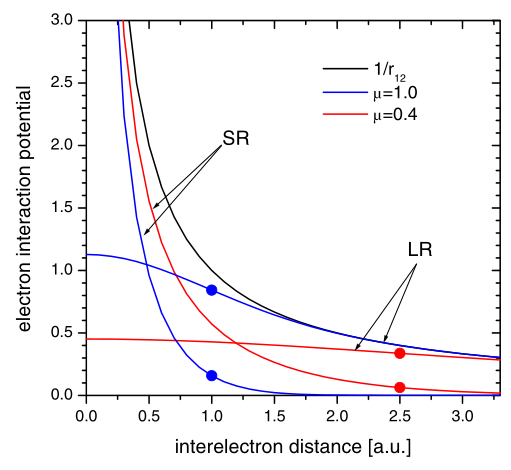
\includegraphics[width=0.4\textwidth]{RangeSeperation.png}
    \caption{Long- and short-range electron interaction potentials, $\frac{\operatorname{erf}(\mu r_{12})}{r_{12}}$} (LR) and $\frac{1-\operatorname{erf}(\mu r_{12})}{r_{12}}$ (SR) for $\mu=1.0$ and $\mu=0.4$. Dots indicate position cutoff radius $r_C=1/\mu$. 
    \label{fig:RangeSeperation}
\end{figure}
\begin{equation}
    \bar{\textbf{H}}=\sum_{m,n=0}^{N-1}\omega^{\prime}_{mn}\sum_{i=0}^{\eta-1}\prod_{b=0}^{\log N-1}\textbf{X}_{i\log N +b}^{m_b}\textbf{Z}_{i\log N+b}^{n_b}+\frac{1}{2}\sum_{m,p=1}^{N-1}\gamma^{\prime}_{mp}\sum_{i\neq j}^{\eta-1}\prod_{b=0}^{\log N-1}\textbf{Z}_{i\log N+b}^{m_b}\textbf{Z}_{j\log N+b}^{p_b},
\end{equation}
where
\begin{equation}
    \omega^{\prime}_{mn}=
    \begin{cases}
        0 \quad \text{if} \, m=n=0, \\
        \omega_{0n}+(N-1)\gamma_{0n} \quad \text{if} \, m=0, n\neq0,\\
        \omega_{mn} \quad \text{otherwise}.
    \end{cases}
\end{equation}
\begin{equation}
    \gamma^{\prime}_{mp}=
    \begin{cases}
        0\quad \text{if} \, m=0\, \text{or}\, p=0 \\
        \gamma_{mp} \quad \text{otherwise}
    \end{cases}
\end{equation}
\section{Quadratic Unconstrained Binary Optimization (QUBO) and Ising Model}
The following content is from the tutorial held by D-Wave \cite{DWAVE_Tutorial}. In the context of D-Wave's quantum annealing, QUBO and the Ising model are the two primary mathematical frameworks used to formulate optimization problems. Both are unified under the broader category of \textbf{Binary Quadratic Models (BQM)}.
QUBO model can be used to a wide range of optimization problems, including combinatorial optimization, machine learning, and constraint satisfaction problems. The QUBO formulation is particularly useful in quantum computing and optimization, as it can be directly mapped to the hardware of quantum annealers like those developed by D-Wave.
QUBO is a mathematical representation of an optimization problem where the objective function is a quadratic polynomial of binary variables. The goal is to find the assignment of these binary variables that minimizes (or maximizes) the objective function. 
Unconstrained means that there are no explicit constraints on the variables, allowing for a more flexible formulation of problems. The QUBO formulation is particularly useful in quantum computing and optimization, as it can be directly mapped to the hardware of quantum annealers like those developed by D-Wave.
\subsection{QUBO Formulation}
Because $x^2 = x$ for binary variables, the QUBO formulation can be expressed as:
\begin{equation}
\min_{x \in \{0,1\}^n} x^T Q x
\label{eqn:qubo}
\end{equation}
where $x$ is a vector of binary variables, and $Q$ is an upper triangular matrix that defines the coefficients of the quadratic terms. The elements of $Q$ represent the interactions between the binary variables, and the diagonal elements represent the linear terms.
Here are some specific examples of QUBO formulations for numbers of varaibles:
\begin{itemize}
\item One-variable QUBO: $Q = [1]$, the objective function is $f(x) = x$.
\item Two-variable QUBO: $Q = \begin{bmatrix} 1 & 2 \\ 0 & 3 \end{bmatrix}$, the objective function is $f(x_1, x_2) = x_1 + 2x_1x_2 + 3x_2$.
\item Three-variable QUBO: $Q = \begin{bmatrix} 1 & 2 & 3 \\ 0 & 4 & 5 \\ 0 & 0 & 6 \end{bmatrix}$, the objective function is $f(x_1, x_2, x_3) = x_1 + 2x_1x_2 + 3x_1x_3 + 4x_2 + 5x_2x_3 + 6x_3$.
\end{itemize}
It is easy to see that the number contained in the QUBO matrix $Q$ corresponds to the coefficients of the objective function. In contrast, the following examples are NOT QUBOs:
\begin{itemize}
    \item $f(x_1) = 3x_1 + 4 + x_1^3$
    \item $f(x_1, x_2) = 11 + 2.7x_1 - 3x_2 + 9.3x_1/x_2$
    \item $f(x_1, x_2, x_3) = x_1x_2x_3$
\end{itemize}
Except for the $Q$ matrix, the QUBO can also be represented in a graphical form, where each variable is represented as a node, and the edges denote the interactions between the variables. The weights of the edges correspond to the coefficients in the QUBO matrix. This graphical representation can be useful for visualizing the structure of the optimization problem and understanding the relationships between the variables. Figure \ref{fig:qubo_graph} is an example of a QUBO graph for the three-variable case $f(x_1, x_2, x_3)=x_1 + 2x_1x_2 + 3x_1x_3 + 4x_2 + 5x_2x_3 + 6x_3$. In this graph, constant terms and variable names are omitted, and the weights of the edges are labeled. The nodes represent the binary variables $x_1$, $x_2$, and $x_3$, while the edges represent the interactions between these variables, with their weights corresponding to the coefficients in the QUBO matrix.
\begin{figure}
    \centering
    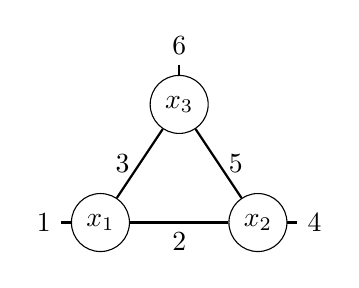
\begin{tikzpicture}
        \node[circle, draw] (x1) at (0, 0) {$x_1$};
        \node[circle, draw] (x2) at (2, 0) {$x_2$};
        \node[circle, draw] (x3) at (1, 1.5) {$x_3$};

        \draw[thick] (x1) -- (x2) node[midway, below] {2};
        \draw[thick] (x1) -- (x3) node[midway, left] {3};
        \draw[thick] (x2) -- (x3) node[midway, right] {5};

        \draw[thick] (x1) -- ++(-0.5, 0) node[left] {1};
        \draw[thick] (x2) -- ++(0.5, 0) node[right] {4};
        \draw[thick] (x3) -- ++(0, 0.5) node[above] {6};
    \end{tikzpicture}
    \caption{Example of a QUBO graph}\label{fig:qubo_graph}
\end{figure}

\subsection{Ising Model}
The Ising model is a mathematical model used to describe the behavior of ferromagnetic materials. It is closely related to the QUBO formulation and can be used to represent optimization problems in a different but equivalent way. In the Ising model, the variables are spins that can take values of either +1 or $-1$, and the interactions between spins are represented by coupling constants. The goal is to find the configuration of spins that minimizes the energy of the system. 
The mathematical representation of the Ising model can be expressed as:
\begin{equation}
\min_{s \in \{-1, 1\}^n} s^T J s + h^T s
\label{eqn:ising}
\end{equation}
where $s$ is a vector of spin variables, $J$ is a matrix that defines the coupling constants between spins, and $h$ is a vector that represents the external magnetic field. The first term represents the interactions between spins, while the second term represents the influence of the external field on the spins.

Compared to the QUBO formulation Eqn \ref{eqn:qubo}, the Ising model uses spin variables instead of binary variables. However, there is a direct mapping between the two formulations, allowing for the conversion of problems from one representation to the other. The relationship between the QUBO and Ising model can be established through a simple transformation of variables, enabling the use of either framework depending on the specific requirements of the optimization problem at hand.

\subsection{Application of QUBO and Ising model}
Then, what type of computational problems can be solved using QUBO and Ising models?
QUBO and Ising models can be used to solve a wide range of computational problems, including but not limited to ~\cite{Lucas_2014}:
\begin{enumerate}
    \item  Combinatorial Optimization: Problems such as the traveling salesman problem, graph coloring, and maximum cut can be formulated as QUBO or Ising problems, allowing for efficient exploration of the solution space.
    \item  Machine Learning: QUBO and Ising models can be applied to various machine learning tasks, such as feature selection, clustering, and training of certain types of neural networks, by formulating the learning objectives as optimization problems.
    \item  Constraint Satisfaction Problems: Many constraint satisfaction problems, such as satisfiability (SAT) and scheduling problems, can be expressed in QUBO or Ising form, enabling the use of quantum annealing or other optimization techniques to find feasible solutions.
\end{enumerate}
\appendix

\section{Derivation of Formulae}
\renewcommand{\theequation}{\thesection.\arabic{equation}}
\setcounter{equation}{0}
\subsection{Laplacian of two electron system}
\label{subsec:Laplacian}
The following derivation is for the Eqn. (2) in \cite{giner2021transcorrelated}, which is Eqn.~(\ref{eqn:HeliumHamiltonian}) here. It is about the Hamiltonian of the helium atom using $r_i=|\textbf{r}_i|$ and $r_{12}=|\textbf{r}_1-\textbf{r}_2|$ coordinates
\begin{equation}
    H=h_c+\frac{1}{r_{12}}
\end{equation}
where 
\begin{equation}
    \begin{split}
        h_c=&-\frac{1}{2}\sum_{i=1}^{2}\left(\frac{\partial^2}{\partial r_i^2}+\frac{2}{r_i}\frac{\partial}{\partial r_i}+\frac{2Z}{r_i}\right)-\left(\frac{\partial^2}{\partial r_{12}^2}+\frac{2}{r_{12}}\frac{\partial}{\partial r_{12}}\right) \\
        &-\left(\frac{\textbf{r}_1}{r_1}\cdot\frac{\textbf{r}_{12}}{r_{12}}\frac{\partial}{\partial r_1}+\frac{\textbf{r}_2}{r_2}\cdot\frac{\textbf{r}_{21}}{r_{21}}\frac{\partial}{\partial r_2}\right).
    \end{split}    
    \label{eqn:HeliumHamiltonian}
\end{equation}
Suppose $f(r)$ is a scalar function of $r$, then
\begin{equation}
    \nabla\cdot\left(\hat{\textbf{r}}f(r)\right)=\frac{\partial}{\partial x}\left(\frac{x}{r}f(r)\right)+\frac{\partial}{\partial y}\left(\frac{y}{r}f(r)\right)+\frac{\partial}{\partial z}\left(\frac{z}{r}f(r)\right).
\end{equation}
Let us concentrate on $\frac{\partial}{\partial x}\left(\frac{x}{r}f(r)\right)$ first, it can be expanded into 
\begin{equation}
    \frac{\partial}{\partial x}\left(\frac{x}{r}f(r)\right)=\frac{\partial}{\partial x}\left(\frac{x}{r}\right)f(r)+\frac{x}{r}\frac{\partial}{\partial x}\left(f(r)\right).
\end{equation}
Considering $r=\sqrt{x^2+y^2+z^2}$, we have $\frac{\partial}{\partial x}(\frac{x}{r})=\frac{y^2+z^2}{r^3}$ and $\frac{\partial}{\partial x}(f(r))=\frac{\partial f}{\partial r}\frac{\partial r}{\partial x}=\frac{x}{r}\frac{\partial f}{\partial r}$. Therefore, we obtain
\begin{equation}
    \frac{\partial}{\partial x}\left(\frac{x}{r}f(r)\right)=\frac{y^2+z^2}{r^3}f(r)+\frac{x^2}{r^2}\frac{\partial f}{\partial r}
    \label{eqn:theFirstTerm}
\end{equation}
The other two terms can be handled in the same way, and we get 
\begin{equation}
    \frac{\partial}{\partial y}\left(\frac{y}{r}f(r)\right)=\frac{x^2+z^2}{r^3}f(r)+\frac{y^2}{r^2}\frac{\partial f}{\partial r}
    \label{eqn:theSecondTerm}
\end{equation}
and
\begin{equation}
    \frac{\partial}{\partial z}\left(\frac{z}{r}f(r)\right)=\frac{x^2+y^2}{r^3}f(r)+\frac{z^2}{r^2}\frac{\partial f}{\partial r}.
    \label{eqn:theThirdTerm}
\end{equation}
From Eqn. (\ref{eqn:theFirstTerm}), (\ref{eqn:theSecondTerm}) and (\ref{eqn:theThirdTerm}), we eventually reach
\begin{equation}
    \nabla\cdot\left(\hat{\textbf{r}}f(r)\right)=\frac{2}{r}f(r)+\frac{\partial f}{\partial r}.
    \label{eqn:FirstOrderofNabla}
\end{equation}
Based on the coordinates we are using, we have 
\begin{equation}
    \nabla_1\cdot\nabla_1=\nabla_1\cdot\left(\hat{\textbf{r}}_1\frac{\partial\psi}{\partial r_1}\right)+\nabla_1\cdot\left(\hat{\textbf{r}}_{12}\frac{\partial\psi}{\partial r_{12}}\right).
    \label{eqn:SecondNabla}
\end{equation}
Using Eqn. (\ref{eqn:FirstOrderofNabla}), the first term on the right side of Eqn. (\ref{eqn:SecondNabla}) can be written into
\begin{equation}
    \nabla_1\cdot\left(\hat{\textbf{r}}_1\frac{\partial\psi(r)}{\partial r_1}\right)=\frac{2}{r_1}\psi(r)+\frac{\partial\psi(r)}{\partial r_1}\rightarrow\left(\frac{2}{r_1}\frac{\partial}{\partial r_1}+\frac{\partial^2}{\partial r_1^2}\right)\psi(r),
    \label{eqn:secondNablaonr_1a}
\end{equation}
where $r$ is used to denote the whole coordinates ($r_1, r_2, r_{12}$).
As to the second term on the right side of Eqn. (\ref{eqn:SecondNabla}), it is 
\begin{equation}
    \begin{split}
        \nabla_1\cdot\left(\hat{\textbf{r}}_{12}\frac{\partial\psi}{\partial r_{12}}\right)=&\frac{\partial}{\partial x_1}\left(\frac{x_1-x_2}{r_{12}}\frac{\partial\psi(r)}{\partial r_{12}}\right) \\
        &+\frac{\partial}{\partial y_1}\left(\frac{y_1-y_2}{r_{12}}\frac{\partial\psi(r)}{\partial r_{12}}\right)+\frac{\partial}{\partial z_1}\left(\frac{z_1-z_2}{r_{12}}\frac{\partial\psi(r)}{\partial r_{12}}\right)
    \end{split}
    \label{eqn:secondNabla_2}    
\end{equation}
where $r_{12}=\sqrt{(x_1-x_2)^2+(y_1-y_2)^2+(z_1-z_2)^2}$, which is a function of $x_1, x_2, y_1, y_2, z_1, z_2$. Therefore, we need the chain rule to perform the derivative. Let's start with the first term on the right side of Eqn. (\ref{eqn:secondNabla_2}):
\begin{equation}
    \begin{split}
        &\frac{\partial}{\partial x_1}\left(\frac{x_1-x_2}{r_{12}}\frac{\partial\psi}{\partial r_{12}}\right)  \\
        &=\frac{\partial}{\partial x_1}\left(\frac{x_1-x_2}{r_{12}}\right)\frac{\partial\psi}{\partial r_{12}}+\frac{x_1-x_2}{r_{12}}\frac{\partial}{\partial x_1}\left(\frac{\partial\psi}{\partial r_{12}}\right) \\
        &=\left[\frac{1}{r_{12}}-\frac{(x_1-x_2)^2}{r_{12}^3}\right]\frac{\partial\psi}{\partial r_{12}}+\frac{x_1-x_2}{r_{12}}\left[\frac{\partial^2\psi}{\partial r_1\partial r_{12}}\frac{\partial r_1}{\partial x_1}+\frac{\partial^2\psi}{\partial r_{12}^2}\frac{\partial r_{12}}{\partial x_1}\right] \\
        &=\frac{(y_1-y_2)^2+(z_1-z_2)^2}{r_{12}^3}\frac{\partial\psi}{\partial r_{12}}+\frac{x_1(x_1-x_2)}{r_1r_{12}}\frac{\partial^2\psi}{\partial r_1\partial r_{12}}+\frac{(x_1-x_2)^2}{r_{12}^2}\frac{\partial^2\psi}{\partial r^2_{12}}.
    \end{split}
    \label{eqn:A_11_1}
\end{equation}
Similarly, we have
\begin{equation}
    \begin{split}
        &\frac{\partial}{\partial y_1}\left(\frac{y_1-y_2}{r_{12}}\frac{\partial\psi(r)}{\partial r_{12}}\right) \\
        &=\frac{(x_1-x_2)^2+(z_1-z_2)^2}{r_{12}^3}\frac{\partial\psi}{\partial r_{12}}+\frac{y_1(y_1-y_2)}{r_1r_{12}}\frac{\partial^2\psi}{\partial r_1\partial r_{12}}+\frac{(y_1-y_2)^2}{r_{12}^2}\frac{\partial^2\psi}{\partial r^2_{12}}
    \end{split}
    \label{eqn:A_11_2}
\end{equation}
and
\begin{equation}
    \begin{split}
        &\frac{\partial}{\partial z_1}\left(\frac{z_1-z_2}{r_{12}}\frac{\partial\psi(r)}{\partial r_{12}}\right) \\
        &=\frac{(x_1-x_2)^2+(y_1-y_2)^2}{r_{12}^3}\frac{\partial\psi}{\partial r_{12}}+\frac{z_1(z_1-z_2)}{r_1r_{12}}\frac{\partial^2\psi}{\partial r_1\partial r_{12}}+\frac{(z_1-z_2)^2}{r_{12}^2}\frac{\partial^2\psi}{\partial r^2_{12}}.
    \end{split}
    \label{eqn:A_11_3}
\end{equation}
Sum up Eqns (\ref{eqn:A_11_1}, \ref{eqn:A_11_2}) and (\ref{eqn:A_11_3}), we can rewrite Eqn. (\ref{eqn:secondNabla_2}) into
\begin{equation}
    \nabla_1\cdot\left(\hat{\textbf{r}}_{12}\frac{\partial\psi}{\partial r_{12}}\right)=\frac{2}{r_{12}}\frac{\partial\psi}{\partial r_{12}}+\hat{\textbf{r}}_1\cdot\hat{\textbf{r}}_{12}\frac{\partial^2\psi}{\partial r_1\partial r_{12}}+\frac{\partial^2\psi}{\partial r^2_{12}}.
    \label{eqn:secondNabla_part2}
\end{equation}
Now, after substituting Eqn. (\ref{eqn:secondNablaonr_1a}) and Eqn. (\ref{eqn:secondNabla_part2}) into Eqn. (\ref{eqn:SecondNabla}), we get
\begin{equation}
    \nabla_1\cdot\nabla_1\psi=\frac{2}{r_1}\frac{\partial\psi}{\partial r_1}+\frac{\partial^2\psi}{\partial r_1^2}+\frac{2}{r_{12}}\frac{\partial\psi}{\partial r_{12}}+\hat{\textbf{r}}_1\cdot\hat{\textbf{r}}_{12}\frac{\partial^2\psi}{\partial r_1\partial r_{12}}+\frac{\partial^2\psi}{\partial r^2_{12}}
    \label{eqn:Laplacian_1}
\end{equation}
Repeat the same procedures, we can find the expansion of $\nabla_2\cdot\nabla_2$, which is
\begin{equation}
    \nabla_2\cdot\nabla_2\psi=\frac{2}{r_2}\frac{\partial\psi}{\partial r_2}+\frac{\partial^2\psi}{\partial r_2^2}+\frac{2}{r_{12}}\frac{\partial\psi}{\partial r_{12}}+\hat{\textbf{r}}_2\cdot\hat{\textbf{r}}_{12}\frac{\partial^2\psi}{\partial r_2\partial r_{12}}+\frac{\partial^2\psi}{\partial r^2_{12}}
    \label{eqn:Laplacian_2}
\end{equation}
Join Eqn. (\ref{eqn:Laplacian_1}) and Eqn. (\ref{eqn:Laplacian_2}) together, we can recover the Eqn. (45a) in \cite{HYLLERAAS19641}, which is
\begin{equation}
    \begin{split}
        \nabla_1^2\psi+\nabla_2^2\psi&=\frac{\partial^2\psi}{\partial r_1^2}+\frac{2}{r_1}\frac{\partial\psi}{\partial r_1}+\frac{\partial^2\psi}{\partial r_2^2}+\frac{2}{r_2}\frac{\partial\psi}{\partial r_2}+2\frac{\partial^2\psi}{\partial r_{12}^2} \\
        &+\frac{4}{r_{12}}\frac{\partial\psi}{\partial r_{12}}+\hat{\textbf{r}}_1\cdot\hat{\textbf{r}}_{12}\frac{\partial^2\psi}{\partial r_1\partial r_{12}}+\hat{\textbf{r}}_2\cdot\hat{\textbf{r}}_{12}\frac{\partial^2\psi}{\partial r_2\partial r_{12}}.
    \end{split}
\end{equation}
% \begin{equation}
%     \underbrace{a + b + c}_{\phantom{xx}\text{注释}}
% \end{equation}
\subsection{Exponentiate Matrix}
If we have a real number $x$ and a matrix $A$ such that $A^2=I$, we can prove
\begin{equation}
    \exp(iAx)=\cos(x)I+i\sin(x)A.
    \label{eqn:ExponentiateMatrix}
\end{equation}
Making use of the Taylor expansion of exponential function 
\begin{equation}
    e^x=\sum_{n=0}^{\infty}\frac{x^n}{n!}=1+x+\frac{x^2}{2!}+\frac{x^3}{3!}+\frac{x^4}{4!}+\cdots,
    \label{eqn:TaylorExp}
\end{equation}
we get
\begin{equation}
    \begin{split}
        \exp(iAx)&=1+iAx+\frac{(iAx)^2}{2!}+\frac{(iAx)^3}{3!}+\frac{(iAx)^4}{4!}+\cdots\\
        &=1+iAx-\frac{x^2}{2!}I-\frac{iAx^3}{3!}+\frac{x^4}{4!}I+\frac{iAx^5}{5!}+\cdots\\
        &=\cos(x)I+i\sin(x)A.
    \end{split}
\end{equation}
With Eqn.~(\ref{eqn:ExponentiateMatrix}), we can easily understand the property of \textit{rotation operators} about $\hat{x},\hat{y}$ and $\hat{z}$:
\begin{equation}
    R_x(\theta)\equiv e^{-i\theta X/2}=\cos\left(\frac{\theta}{2}\right)I-i\sin\left(\frac{\theta}{2}\right)X=\begin{bmatrix}
        \cos\frac{\theta}{2}&-i\sin\frac{\theta}{2}\\-i\sin\frac{\theta}{2}&\cos\frac{\theta}{2}
    \end{bmatrix}
\end{equation}
\begin{equation}
    R_y(\theta)\equiv e^{-i\theta Y/2}=\cos\left(\frac{\theta}{2}\right)I-i\sin\left(\frac{\theta}{2}\right)Y=\begin{bmatrix}
        \cos\frac{\theta}{2}&-\sin\frac{\theta}{2}\\\sin\frac{\theta}{2}&\cos\frac{\theta}{2}
    \end{bmatrix}
\end{equation}
\begin{equation}
    R_z(\theta)\equiv e^{-i\theta Z/2}=\cos\left(\frac{\theta}{2}\right)I-i\sin\left(\frac{\theta}{2}\right)Z=\begin{bmatrix}
        e^{-i\theta/2}&0\\0&e^{i\theta/2}.
    \end{bmatrix}
\end{equation}
If the rotation by $\theta$ is about a real unit vector $\hat{n}=(n_x, n_y, n_z)$, the epxpressions can be generalized into 
\begin{equation}
    R_{\hat{n}}(\theta)\equiv\exp(-i\theta\hat{n}\cdot\vec{\sigma}/2)=\cos\left(\frac{\theta}{2}\right)I-i\sin\left(\frac{\theta}{2}\right)(n_xX+n_yY+n_zZ).
\end{equation}
Now, let's talk about another topic: \textbf{Baker-Campbell-Hausdorf formula} (BCH), which is usually expressed as
\begin{equation}
    e^Xe^Y=e^Z,
    \label{eqn:BCH1}
\end{equation}
where 
\begin{equation}
    Z=X+Y+\frac{1}{2}[X,Y]+\frac{1}{12}\left[X,[X,Y]\right]-\frac{1}{12}\left[Y,[X,Y]\right]+\cdots.
    \label{eqn:Z}
\end{equation}
To prove Eqn.~(\ref{eqn:BCH1}), we need to make use the following Taylor's expansion:
\begin{equation}
    \ln(1+x)=x-\frac{x^2}{2}+\frac{x^3}{3}-\frac{x^4}{4}+\cdots+(-1)^{n+1}\frac{x^n}{n}+\cdots\quad\text{with}\quad-1<x\le 1.
    \label{eqn:TaylorLn1+x}
\end{equation}
Applying Eqn.~(\ref{eqn:TaylorExp}) onto $e^X$ and $e^Y$, and multiplying them together, we get
\begin{equation}
    \begin{split}
        e^Xe^Y&=\left(1+X+\frac{X^2}{2!}+\frac{X^3}{3!}+\frac{X^4}{4!}+\cdots\right)\left(1+Y+\frac{Y^2}{2!}+\frac{Y^3}{3!}+\frac{Y^4}{4!}+\cdots\right)\\
        &=1+Y+X+\frac{Y^2}{2!}+XY+\frac{X^2}{2!}+\frac{Y^3}{3!}+\frac{XY^2}{2!}+\frac{X^2Y}{2!}+\frac{X^3}{3!}+\frac{Y^4}{4!}+\frac{XY^3}{3!}\\
        &+\frac{X^2Y^2}{2!2!}+\frac{X^3}{3!}Y+\frac{X^4}{4!}+\cdots.
    \end{split}
\end{equation}
If we only care about the order only to three, we can let $x=Y+X+\frac{Y^2}{2!}+XY+\frac{X^2}{2!}+\frac{Y^3}{3!}+\frac{XY^2}{2!}+\frac{X^2Y}{2!}+\frac{X^3}{3!}$ so that we can use Eqn.~(\ref{eqn:TaylorLn1+x}) to figure out the result of expanding $\ln(e^Xe^Y)$ to the power of three. After \href{https://www.youtube.com/watch?v=vt3_uYU98RI}{some tedious algebraic processes}, we can recover the result identical to Eqn.~(\ref{eqn:Z}).

However, the Eqn. (29) in \cite{feniou2025realspacechemistryquantumcomputers} is NOT directly from the BCH formula presented here. It is obtained from the same idea we obtain the BCH: expansion of the exponential function to the order we need (here we approximate to the order of 2 for $\tau$).
\begin{equation}
    \begin{split}
        \tilde{H} &\coloneqq e^{-\tau}\hat{H}e^{\tau} \\
        &=\left(1-\tau+\frac{\tau^2}{2!}\right)\hat{H}\left(1+\tau+\frac{\tau^2}{2}\right) \\
        &=\hat{H}+\hat{H}\tau+\hat{H}\frac{\tau^2}{2}-\tau\hat{H}-\tau\hat{H}\tau+\frac{\tau^2}{2}\hat{H} \\
        &=\hat{H}+[\hat{H},\tau]+\frac{1}{2}\left[[\hat{H},\tau],\tau\right].
    \end{split}
    \label{eqn:TruncatSecondOrder}
\end{equation}

\section{Special Functions}
\renewcommand{\theequation}{\thesection.\arabic{equation}}
\setcounter{equation}{0}
This appendix collects special functions used in the note.


\subsection{Chebyshev Polynomials}\label{subsec:Cheby}
The \textit{first kind of Chebyshev polynomial} over the real interval $[-1;1]$ is defined as 
\begin{equation}
    \textbf{T}_j(x)\coloneqq\cos (j \arccos(x)).
    \label{eqn:FirstChebyDef}
\end{equation}
Let $\theta=\arccos(x)$, note that
\begin{equation}
    \cos(j\theta)=\sum_{\substack{0 \le k \le j \\ k \text{ is even}}}\binom{j}{k}i^k\cos^{j-k}(\theta)(1-\cos^2(\theta))^{k/2},
    \label{eqn:ExpanCosjtheta}
\end{equation}
 we can see Eqn.~(\ref{eqn:FirstChebyDef}) can be written into
 \begin{equation}
    \textbf{T}_j(x)=\sum_{\substack{0 \le k \le j \\ k \text{ is even}}}\binom{j}{k}i^k x^{j-k}(1-x^2)^{k/2},
    \label{eqn:FirtChebExpansionForm}
 \end{equation}
 with which we can see $\textbf{T}_j(x)$ is indeed a polynomial. By the way, to prove Eqn.~(\ref{eqn:ExpanCosjtheta}), we need to realize, according to Euler's equation, we have 
 \begin{equation}
    \cos(j\theta)=\Re[(\cos\theta+i\sin\theta)^j].
 \end{equation}

 Now, let's consider the power series $\sum_{j=0}^{\infty}\textbf{T}_j(x)y^j$ generated by the Chebyshev polynomial. Assumming $|y|<1$, we have 
 \begin{equation}
    \begin{split}
        \sum_{j=0}^{\infty}\textbf{T}_j(x)y^j &=\sum_{j=0}^{\infty}\cos(j\theta)y^j=\sum_{j=0}^{\infty}\frac{e^{ij\theta+}+e^{-ij\theta}}{2}y^j\\
        &=\frac{\frac{1}{1-ye^{i\theta}}+\frac{1}{1-ye^{-i\theta}}}{2}=\frac{1-yx}{1+y^2-2yx}
    \end{split}
 \end{equation}
 Sometimes, we use rescaled first Chebyshev polynomial by a factor of 1/2:
 \begin{equation}
    \tilde{\textbf{T}}_j(x)=
    \begin{cases}
        \textbf{T}_j(x), \quad j\ge 1, \\
        \frac{1}{2}\textbf{T}_0(x), \quad j=0.
    \end{cases}
 \end{equation}
In this case, the alternative generative function is
\begin{equation}
    \sum_{j=0}^{\infty}\tilde{\textbf{T}}_j(x)y^j=\frac{1}{2}+\sum_{j=1}^{\infty}\textbf{T}_j(x)y^j=\frac{1-y^2}{2(1+y^2-2yx)}.
\end{equation}
The \textit{Chebyshev polynomial of the second kind} is defined as
\begin{equation}
    \textbf{U}_j(x)\coloneqq\frac{\sin((j+1)\arccos(x))}{\sin(\arccos(x))},
\end{equation}
which has the generating function for $|y|<1$
\begin{equation}
    \sum_{j=0}^{\infty}\textbf{U}_j(x)y^j=\frac{1}{1+y^2-2yx}.
\end{equation}
The two kinds of Chebyshev polynomial are related as the solutions of the Pell equation
\begin{equation}
    \textbf{T}^2_j(x)-(x^2-1)\textbf{U}_{j-1}^2(x)=1.
\end{equation}
The orthogonal relation between the Chebyshev polynomials is
\begin{equation}
    \int_{-1}^{1}\textbf{T}_j(x)\textbf{T}_k(x)\frac{dx}{\sqrt{1-x^2}}=
    \begin{cases}
        0, \quad j\neq k,\\
        \frac{\pi}{2}, \quad j=k\neq0, \\
        \pi, \quad j=k=0.
    \end{cases}
\end{equation}
Therefore, if a function has a Chebyshev expasion
\begin{equation}
    f(x)=\sum_{j=0}^{\infty}\beta_j\textbf{T}_j(x),
\end{equation}
the expansion coefficients must be uniquely determined by
\begin{equation}
    \beta_j=
    \begin{cases}
        \frac{2}{\pi}\int_{-1}^{1}\textbf{T}_j(x)f(x)\frac{dx}{\sqrt{1-x^2}}, \quad j\ge1, \\
        \frac{1}{\pi}\int_{-1}^{1}\textbf{T}_0(x)f(x)\frac{dx}{\sqrt{1-x^2}}, \quad j=0.
    \end{cases}
\end{equation}


\subsection{Error Function} \label{sub:ErrorFun}
The following content are mainly from \href{https://en.wikipedia.org/wiki/Error_function}{Wikipedia}. In mathematics, the \textbf{error function} (also called the \textbf{Gauss error function}), often denoted by \textbf{erf}, is a function $\text{erf}:\mathbb{C}\rightarrow\mathbb{C}$ defined as:
\begin{equation}
    \operatorname{erf}(z)=\frac{2}{\sqrt{\pi}}\int_{0}^{\pi}e^{-t^2}dt.
\end{equation}
In general, this integral is a complex contour integral which is path-independent because $\exp(-t^2)$ is holomorphic on the whole complex plane $\mathbb{C}$. A holomorphic function is a complex-valued function of one or more complex variables that is complex differentiable in a neighbourhood of each point in a domain in complex coordinates space $\mathbb{C}^n$. In many applications, the function argument is a real number, in which case the function value is also real. This nonelementary integral is a sigmoid function that occurs oftern in probability, statistics, and partial differential equations.
\begin{figure}
    \centering
    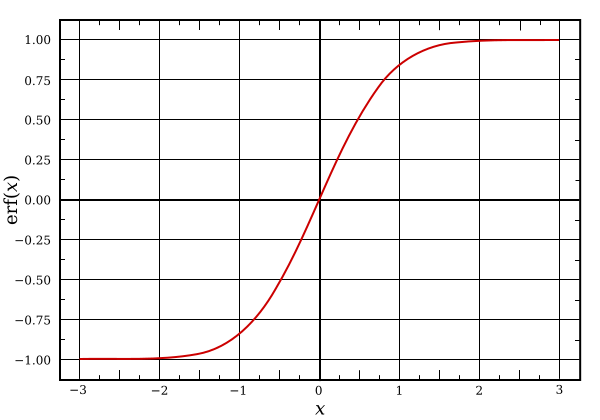
\includegraphics[width=0.4\textwidth]{Error_Function.svg.png}
    \caption{Error Function}
    \label{fig:ErrorFunction}
\end{figure}

In statistics, for non-negative real values of $x$, the error function has the following interpretation: for a real random variable $Y$ which is normally distributed with mean 0 and standard deviation $\frac{1}{\sqrt{2}}$, $\operatorname{erf}(x)$ is the probability that $Y$ falls in the range $[-x, x]$.

Two closely related functions are the \textbf{complementary error function} $\operatorname{erfc}:\mathbb{C}\rightarrow\mathbb{C}$ is defined as
\begin{equation}
    \operatorname{erfc}(z)=1-\operatorname{erf}(z),
\end{equation}
and the \textbf{imaginary error function} $\operatorname{erfi}:\mathbb{C}\rightarrow\mathbb{C}$ is defined as 
\begin{equation}
    \operatorname{erfi}(z)=-i\operatorname{erf}(iz).
\end{equation}
Its derivative is 
\begin{equation}
    \frac{d}{dz}\operatorname{erf}(z)=\frac{2}{\sqrt{\pi}}e^{-z^2}.
\end{equation}
Its antiderivative is
\begin{equation}
    \int\operatorname{erf}(z)dz=z\operatorname{erf}(z)+\frac{e^{-z^2}}{\sqrt{\pi}}+C.
\end{equation}
Its Taylor series expansion is
\begin{equation}
    \operatorname{erf}(z)=\frac{2}{\sqrt{\pi}}\sum_{n=0}^{\infty}\frac{(-1)^n}{2n+1}\frac{z^{2n+1}}{n!}.
\end{equation}
\section{LaTeX 数学符号速查表}
 
\begin{longtable}{|l|p{4cm}|l|p{6cm}|}
\hline
\textbf{类别} & \textbf{命令} & \textbf{效果} \\
\hline
\endfirsthead
\multicolumn{4}{c}{\textit{To be continued}} \\
\hline
\textbf{类别} & \textbf{命令} & \textbf{效果}  \\
\hline
\endhead
\hline
\multicolumn{4}{r}{\textit{Continued on next page}} \\
\endfoot
\hline
\endlastfoot

横线 & \verb|\bar{x}| & $\bar{x}$ \\
     & \verb|\overline{AB}| & $\overline{AB}$ \\
\hline
波浪线 & \verb|\tilde{x}| & $\tilde{x}$  \\
       & \verb|\widetilde{AB}| & $\widetilde{AB}$  \\
\hline
帽子 & \verb|\hat{x}| & $\hat{x}$ \\
     & \verb|\widehat{AB}| & $\widehat{AB}$ \\
\hline
向量 & \verb|\vec{v}| & $\vec{v}$  \\
     & \verb|\bm{v}| & $\bm{v}$  \\
\hline
张量积 & \verb|\otimes| & $\otimes$ \\
       & \verb|\bigotimes_{i=1}^n V_i| & $\bigotimes_{i=1}^n V_i$ \\
\hline
直和 & \verb|\oplus| & $\oplus$ \\
     & \verb|\bigoplus_{i=1}^n V_i| & $\bigoplus_{i=1}^n V_i$ \\
\hline
楔积 & \verb|\wedge| & $\wedge$ \\
~ & \verb|\bigwedge_{i=1}^n \omega_i| & $\bigwedge_{i=1}^n \omega_i$  \\
\hline
定义符号 & \verb|\coloneqq| & $\coloneqq$ \\
\hline
括号 & \verb|\left\{...\right\}| & $\left\{...\right\}$ \\
     & \verb|\Bigg\{...\Bigg\}| & $\Bigg\{...\Bigg\}$  \\
\hline
左尖括号& \verb|\langle| & $\langle$  \\
\hline
花体O& \verb|\mathcal{O}| & $\mathcal{O}$ \\
\hline
范数 & \texttt{\textbackslash|x\textbackslash|} & $\|x\|$ \\
  & \texttt{\textbackslash left\textbackslash| \textbackslash sum\_\{i=1\}\^{}n x\_i \textbackslash right\textbackslash| \_2} & $\left\| \sum_{i=1}^n x_i \right\|_2$ \\
\hline
上确界 & \verb|\sup| & $\sup$ \\
下确界 & \verb|\inf| & $\inf$  \\
\hline
上方括号 & \verb|\lfloor x \rfloor| & $\lfloor x \rfloor$ \\
下方括号 & \verb|\lceil x \rceil| & $\lceil x \rceil$  \\
\hline
分段函数 & \texttt{\textbackslash begin\{cases\} ... \textbackslash end\{cases\}}  & $f(x) = \begin{cases} x^2 & \text{当 } x \geq 0 \\ -x  & \text{当 } x < 0\end{cases}$  \\
\hline
方括号矩阵&\texttt{\textbackslash begin\{bmatrix\} ... \textbackslash end\{bmatrix\}} & $\begin{bmatrix}
     1&1\\1&1
\end{bmatrix}$  \\
\hline
分段长公式 & \texttt{\textbackslash begin\{split\}...\textbackslash end\{split\}} &
$\begin{aligned}
x &= ... \\
  &= ...
\end{aligned}$  \\
\hline
水平省略号 & \texttt{\textbackslash cdots} & $\cdots$ \\
垂直省略号 & \texttt{\textbackslash vdots} & $\vdots$  \\
对角省略号 & \texttt{\textbackslash ddots} & $\ddots$  \\
自动省略号 & \texttt{\textbackslash dots} & $\dots$  \\
加法省略号 & \texttt{\textbackslash dotsb} & $a_1 + a_2 + \dotsb + a_n$ \\
逗号省略号 & \texttt{\textbackslash dotsc} & $a_1, a_2, \dotsc, a_n$ \\
乘法省略号 & \texttt{\textbackslash dotsm} & $a_1 a_2 \dotsm a_n$ \\
积分省略号 & \texttt{\textbackslash dotsi} & $\int \dotsi \int$ \\
其他省略号 & \texttt{\textbackslash dotso} & $\dotso$ \\
\hline
无序列表 & \parbox[t]{4cm}{\texttt{\textbackslash begin\{itemize\}}\\...\texttt{\textbackslash end\{itemize\}}} & \parbox[t]{4.5cm}{\begin{itemize}\item 项目一\item 项目二\end{itemize}}  \\
有序列表 & \parbox[t]{4cm}{\texttt{\textbackslash begin\{enumerate\}}\\...\texttt{\textbackslash end\{enumerate\}}}& \parbox[t]{4.5cm}{\begin{enumerate}\item 项目一\item 项目二\end{enumerate}}  \\
嵌套列表 & \texttt{itemize} 或 \texttt{enumerate} 嵌套使用 & 多层 bullet 或编号 \\
自定义编号 & \texttt{\textbackslash usepackage\{enumitem\}} + \texttt{label=\textbackslash alph*)} 等 & \parbox[t]{4.5cm}{
  \begin{enumerate}[label=\alph*)]
    \item 项目一
    \item 项目二
  \end{enumerate}
} \\
透明占位符 & \texttt{\textbackslash phantom\{内容\}} 或 \texttt{\textasciitilde} & 空白但占位  \\
\hline
结构性注释（下方） & \parbox[t]{4cm}{\texttt{\textbackslash underbrace\{表达式\}\_\{\text\{注释\}\}}} & $\underbrace{a + b + c}_{\text{总项}}$ \\
结构性注释（上方） & \parbox[t]{4cm}{\texttt{\textbackslash overbrace\{表达式\}\^\{\text\{注释\}\}}} & $\overbrace{a + b + c}^{\text{总项}}$ \\
\hline
数学右箭头 & \texttt{\textbackslash rightarrow} & \(\rightarrow\) \\
数学左箭头 & \texttt{\textbackslash leftarrow} & \(\leftarrow\)\\
双向箭头 & \texttt{\textbackslash leftrightarrow} & \(\leftrightarrow\)  \\
长右箭头 & \texttt{\textbackslash longrightarrow} & \(\longrightarrow\) \\
长左箭头 & \texttt{\textbackslash longleftarrow} & \(\longleftarrow\)  \\
长双向箭头 & \texttt{\textbackslash longleftrightarrow} & \(\longleftrightarrow\)\\
右双箭头 & \texttt{\textbackslash Rightarrow} & \(\Rightarrow\)  \\
左双箭头 & \texttt{\textbackslash Leftarrow} & \(\Leftarrow\)  \\
双向双箭头 & \texttt{\textbackslash Leftrightarrow} & \(\Leftrightarrow\)  \\
向上箭头 & \texttt{\textbackslash uparrow} & \(\uparrow\) \\
向下箭头 & \texttt{\textbackslash downarrow} & \(\downarrow\) \\
上下箭头 & \texttt{\textbackslash updownarrow} & \(\updownarrow\) \\
双向上下箭头 & \texttt{\textbackslash Updownarrow} & \(\Updownarrow\) \\
带标签箭头 & \texttt{\textbackslash xrightarrow\{标签\}} & \(\xrightarrow{f}\)  \\
带标签左箭头 & \texttt{\textbackslash xleftarrow\{标签\}} & \(\xleftarrow{g}\)  \\
\hline
带圈符号（基础） & \verb|\odot| & $\odot$ & 小圆圈中有点（你最常用的） \\ 
\hline 带圈符号（基础） & \verb|\oplus| & $\oplus$ & 圆圈加号，直和、XOR \\ 
\hline 带圈符号（基础） & \verb|\ominus| & $\ominus$ & 圆圈减号 \\ 
\hline 带圈符号（基础） & \verb|\otimes| & $\otimes$ & 张量积，Kronecker 积 \\ 
\hline 带圈符号（基础） & \verb|\oslash| & $\oslash$ & 圆圈除号 \\ \hline 带圈符号（基础） & \verb|\circ| & $\circ$ & 小圆圈，函数复合 \\ 
\hline 带圈符号（基础） & \verb|\bigcirc| & $\bigcirc$ & 大圆圈 \\ 
\hline 带圈符号（扩展） & \verb|\circledast| & $\circledast$ & 圆圈星号 \\ 
\hline 带圈符号（扩展） & \verb|\circledcirc| & $\circledcirc$ & 双圈 \\ 
\hline 带圈符号（扩展） & \verb|\circleddash| & $\circleddash$ & 圆圈短横 \\
\hline 文本带圈符号 & \verb|\textcircled{A}| & \textcircled{A} & 文本模式下的带圈字符 \\ 
\hline 自定义带圈符号 & \verb|\tikz \node[circle,draw]{...};| & ○ & 可放任意符号，完全自定义 \\ 
\hline
\end{longtable}

\vspace{1em}
\noindent
\textbf{推荐宏包：} \verb|\usepackage{amsmath, amssymb, bm, mathtools}|


\printbibliography
\end{document}